%% ergebnisse.tex

\chapter{Ergebnisse und Diskussion}
\label{ch:Ergebnisse}
In Abschnitt \ref{sec:datensatz} wird zunächst der berechnete
Datensatz allgemein charakterisiert. Abschnitt
\ref{sec:result-allg-merkm-des} untersucht die Struktur des sich
daraus ergebenden Graphen. Die zeitliche Entwicklung der Gr\"o{\ss}e des
Web of Trust und Statistiken \"uber die Verwendung von Algorithmen
werden in den Abschnitten \ref{sec:result-key-properties} und
\ref{sec:public-key-und} dargestellt. Abschnitt
\ref{sec:result-zusamm-und-comm} analysiert die Community-Struktur der
größten starken Zusammenhangskomponente nach der in Abschnitt
\ref{sec:community-analyse} beschriebenen Vorgehensweise.

\section{Datensatz}
\label{sec:datensatz}

Die Extraktion der hier verwendeten Daten wurde, wie in Abschnitt
\ref{sec:datenextraktion} beschrieben, auf einem vom
Verfasser betriebenen Keyserver am 02.12.2009 vorgenommen. Die
Datenbank des Keyservers war zu diesem Zeitpunkt mit dem Rest des
Keyserver-Netzwerkes vollständig abgeglichen. Der berechnete
Datensatz enthält 2.725.504 Schlüssel und 1.145.337 zugehörige
Signaturen, wobei hier keine Selbstsignaturen enthalten sind. 52.000
Schlüssel wurden während der Extraktion als defekt verworfen. Eine
Stichprobe von 30 verworfenen Schlüssel ergab, dass diese auch von
GnuPG nicht akzeptiert werden, weil sie entweder über keine
UserID-Pakete verfügen oder aus anderen Gründen keine
standardkonformen OpenPGP-Schlüssel darstellen. Von den
nicht-defekten Schlüsseln sind 417.163 Schlüssel abgelaufen und
100.071 Schlüssel wurden zurückgezogen. Die in Relation zur Anzahl
der Schlüssel niedrige Anzahl von Signaturen weist schon darauf hin,
dass ein erheblicher Teil der (gültigen) Schlüssel nicht oder kaum
vernetzt ist. In der Tat verbleiben nach Abzug von Schlüsseln, die
weder ein- noch ausgehende Signaturen haben, nur 325.410 gültige
Schlüssel und 816.785 zugehörige gültige Kanten, die den Graphen
ausmachen.

Die große Mehrheit der im Keyserver-Netzwerk vorhandenen Schlüssel
ist also komplett unvernetzt und nimmt von vorne herein nicht am Web of
Trust teil. Die Überprüfung der Authentizität dieser Schlüssel
anhand öffentlich verfügbarer Informationen ist nicht
möglich. Die Besitzer dieser Schlüssel haben -- sofern sie die
Schlüssel überhaupt einsetzen -- ebenfalls keine Möglichkeit,
die Authentizität anderer Schlüssel zu prüfen. Über die
Gründe für diese geringe Vernetzung kann hier nur spekuliert
werden. Möglich ist etwa, dass die Benutzer schlichtweg keine
Notwendigkeit in der Authentifizierung von Schlüsseln sehen, weil
ihnen Man-in-the-middle und ähnliche Angriffe nicht bekannt sind,
oder das im Web of Trust verwendete Modell zur Verifizierung von
Schlüsseln zu komplex erscheint. Es kann selbstverständlich nicht
ausgeschlossen werden, dass die Verifizierung über Signaturen
läuft, die nicht auf öffentliche Keyserver geladen
wurden. Beachtet werden muss auch, dass der Datensatz keine präzise
Angabe über die momentane Anzahl von PGP-Benutzern erlaubt, da sich
die Schlüssel über einen Zeitraum von 20 Jahren angesammelt haben.

\section{Strukturelle Merkmale des Netzwerkes}
\label{sec:result-allg-merkm-des}

\subsection{Starke Zusammenhangskomponenten}
\label{sec:result-komponentenstruktur}

\begin{figure}[t]
  \centering
  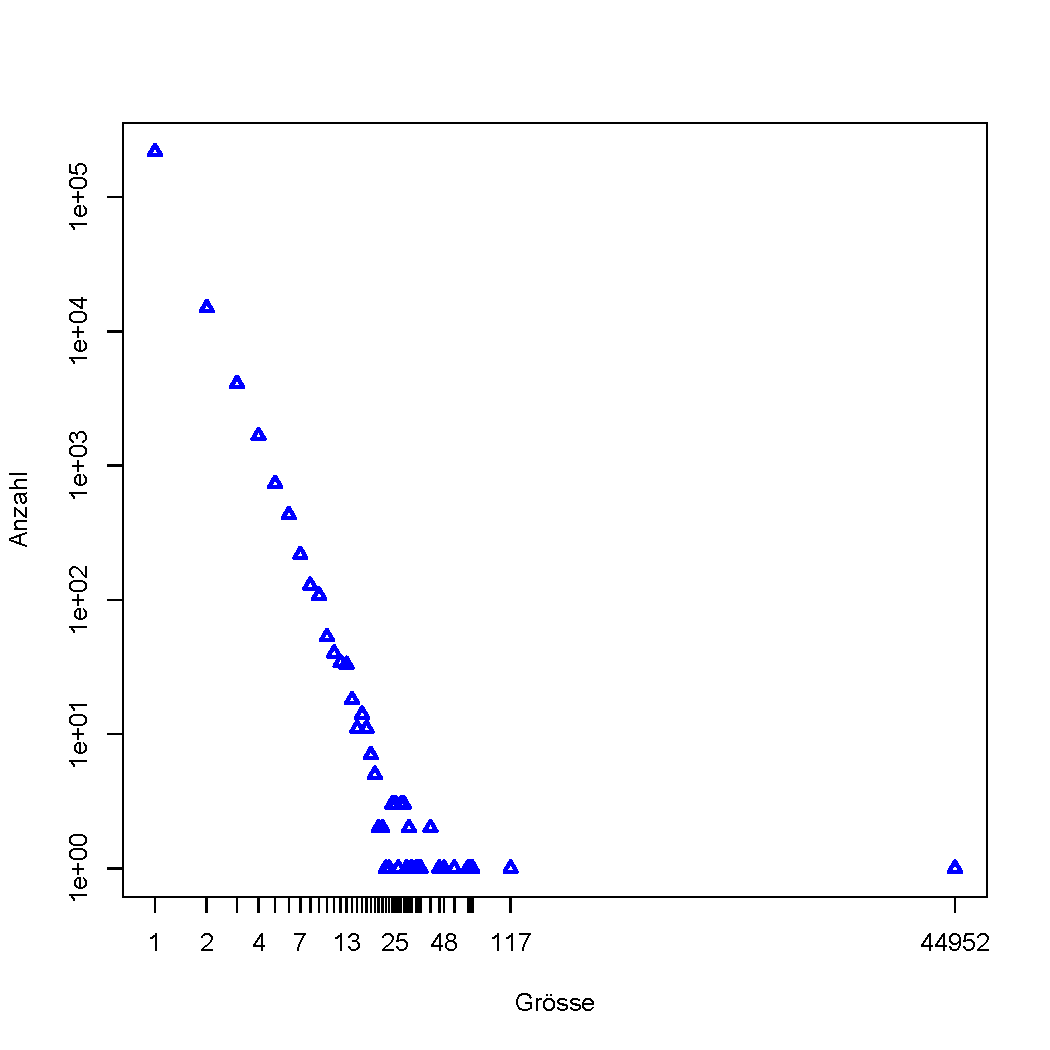
\includegraphics[scale=0.42]{images/component-size.pdf}
  \caption{Größenverteilung der starken Zusammenhangskomponenten}
  \label{fig:component-size}
\end{figure}

Der Graph wurde zunächst in seine 240.382 starken
Zusammenhangskomponenten zerlegt. Die Verteilung der
Größen der Komponenten in Abbildung \ref{fig:component-size} zeigt dabei
zwei Extreme: Es existiert eine einzelne gigantische Komponente mit
ca. 45.000 Knoten. Demgegenüber steht eine geringe Anzahl von kleinen
Komponenten bis zur Größe drei, insbesondere aber deutlich über 100.000
einelementige Komponenten, also einzelne Knoten, die nur
\emph{entweder} ein- oder ausgehende Kanten haben, und über 10.000
zweielementige Komponenten, also durch zwei Kanten verbundene
Knotenpaare. Ein erheblicher Anteil der überhaupt vernetzten Knoten
ist also wiederum nur sehr wenig vernetzt.

\begin{figure}[th!]
  \centering
  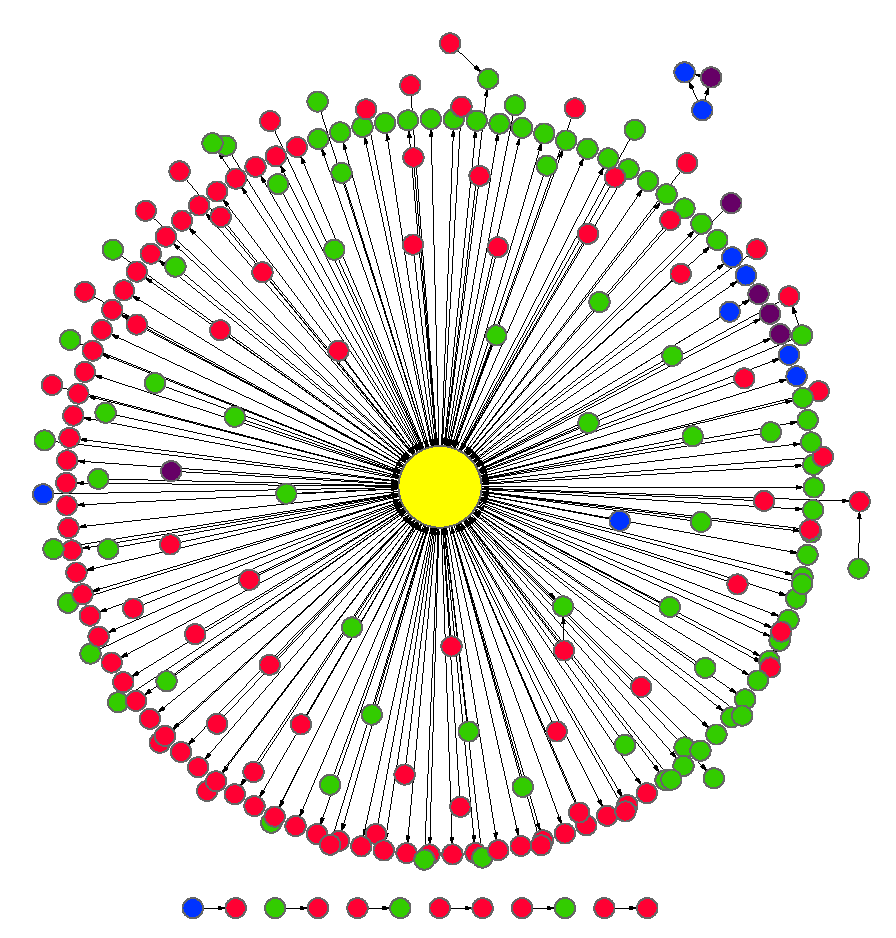
\includegraphics[scale=0.7]{images/component-metagraph-8.pdf}
  \caption{Sternförmige Struktur der starken
    Zusammenhangskomponenten bis zur Größe 6 (rot = Größe 6-10, grün
    = Größe 11-20, blau = Größe 21-30, violett = Größe $>= 31$,
    gelb = MSCC)}
  \label{fig:komponenten-struktur}
\end{figure}

Abbildung \ref{fig:komponenten-struktur} zeigt die Struktur der
Zusammenhangskomponenten bis zur Größe sechs, die mit anderen
Komponenten verbunden sind. Es ergibt sich eine sternförmige
Struktur, bei der die kleineren Komponenten fast ausschließlich mit
der größten Komponente verbunden sind und es so gut wie keine
weitere Vernetzung gibt. Der Aufwand, der nötig ist, um zwei starke
Zusammenhangskomponenten verschmelzen zu lassen, ist sehr gering: dazu
ist nur genau eine Kante in jede Richtung nötig. Je mehr Kanten
(also Signaturen) in eine Richtung verlaufen, desto wahrscheinlicher
ist es, dass es zu einer dieser Kanten auch eine Gegenkante, also eine
entsprechende Signatur in Gegenrichtung, gibt. Es kann also davon
ausgegangen werden, dass die Komponenten nur durch sehr wenige Kanten,
die eben nur in eine Richtung verlaufen können, verbunden
sind. Daraus ergibt sich, dass die Mitglieder der kleinen Komponenten
nur eine sehr geringe Signaturaktivität aufweisen können. Würde
eine nennenswerte Anzahl von Signaturen entstehen, so wäre die
Wahrscheinlichkeit für das Verschmelzen von Komponenten sehr
hoch. Die Anzahl kleiner Komponenten müsste in diesem Fall deutlich
geringer sein.

Die \emph{Nützlichkeit} des Web of Trust für die Teilnehmer, deren
Schlüssel nicht in der größten starken Zusammenhangskomponente
(MSCC)
enthalten sind, ist gering: Die Menge der Schlüssel, die von einem
Teilnehmer anhand von Signaturketten verifiziert werden kann,
beschränkt sich zunächst auf die eigene Komponente und ist damit
sehr klein. Zwar gibt es auch -- wie oben gezeigt -- Vernetzung
zwischen kleineren Komponenten und der größten Komponente. Es
existieren ca. 18.000 Knoten, die Knoten aus der größten Komponente
direkt über eine einzige Kante erreichen können. Allerdings muss
hier beachtet werden, dass das in PGP/GnuPG verwendete
Verifizierungsmodell die Länge der verwendbaren Signaturketten
begrenzt -- in der Standardeinstellung von GnuPG auf die maximale
Länge fünf (siehe Abschnitt
\ref{sec:das-gnupg-vertrauensmodell}). Schon innerhalb der größten
Komponente sind viele kürzeste Pfade länger als dieses Maximum
(siehe Abschnitt \ref{sec:kennz-des-graph}). Durch den zusätzlichen
Schritt zu einem Knoten innerhalb der größten Komponente
verlängert sich der Pfad. Insbesondere wenn es sich bei diesen
Knoten um schwach vernetzte Knoten handelt, die am "`Rand"' der
größten Komponente liegen, ist die Menge der auf Pfaden benutzbarer
Länge erreichbaren Knoten beschränkt. Kann die größte
Komponente nur indirekt über andere Knoten erreicht werden,
reduziert sich diese Menge noch weiter. Gleiches gilt auch für die
Erreichbarkeit der Menge von ca. 92.000 Knoten, zu denen eine Kante von
Knoten der größten Komponente aus besteht. 

Beachtet werden muss
allerdings die Existenz von zentralen Certificate Authorities im
eigentlich dezentralen Web of Trust. Mit den drei seit 1997 im Rahmen
der "`Krypto-Kampagne"' der Zeitschrift c't (siehe Abschnitt
\ref{sec:sozi-komp-des}) verwendeten Zertifizierungsschlüsseln
wurden insgesamt 23.813 derzeit gültige Schlüssel
unterschrieben. Von diesen liegen nur 2.578 Schlüssel innerhalb der
größten Komponente. Wenn also nur dem verwendeten
Zertifizierungsprozess und damit diesen drei
Zertifizierungsschlüsseln vertraut wird, sind immerhin etwa 20.000
Schlüssel außerhalb der größten Komponente verifizierbar. Es
zeigt sich hier auch die Flexibilität des Web of Trust-Konzeptes,
das die Integration von zentralen Komponenten in das eigentlich
dezentrale Netz erlaubt.

Insgesamt lassen diese Daten den Schluss zu, dass ausschließlich die
größte starke Zusammenhangskomponente Schlüssel von Personen
enthält, die sich durch regelmäßige Signaturaktivitäten am Web
of Trust beteiligen und es zur Verifizierung von Schlüsseln
benutzen. 

\subsection{Netzwerkstatistiken der größten starken
  Zusammenhangskomponente}
\label{sec:kennz-des-graph}

Die weitere Untersuchung der Topologie des Graphen konzentriert sich
auf die größte starke Zusammenhangskomponente. Starke
Zusammenhangskomponenten als Einheit der Betrachtung machen Sinn, weil
die Verwendung des Graphen für die Verifizierung von Schlüsseln
gerade die Erreichbarkeit voraussetzt und weil eine Reihe von
Netzwerkstatistiken nur definiert sind, wenn zwischen allen Paaren von
Knoten Pfade existieren. Da im vorherigen Abschnitt argumentiert
wurde, dass die größte starke Zusammenhangskomponente die einzige
ist, die in größerem Maßstab vernetzt ist und in der
Signaturaktivitäten stattfinden, scheint eine Untersuchung der
restlichen Komponenten in diesem Rahmen nicht sinnvoll.

Der induzierte Teilgraph der größten starken
Zusammenhangskomponente besteht aus 44.952 Knoten und 442.960
gerichteten Kanten. Dieser Teilgraph ist deutlich größer als die
bisher in der Literatur verwendeten PGP-Netzwerke:  ein gerichtetes
Netzwerk von ca. 12.000 Knoten bei \cite{Capkun2002} und ein Netzwerk
von 10.700 Knoten, bei dem alle einseitigen Signaturen gelöscht
wurden bei \cite{Boguna2004} und \cite{Gregory2010}. Beide Netzwerke
stellen die größte starke Zusammenhangskomponente dar und wurden im
Jahr 2001 extrahiert.

\subsubsection{Gegenseitigkeit von Kanten}
\label{sec:gegens-von-kant}

Der \emph{Reciprocity}-Wert eines gerichteten Graphen gibt den Anteil
von Kanten an, die in beide Richtungen verlaufen. Für die größte
Komponente ist dieser Wert 0,510. Das bedeutet, dass es für eine
gegebene Kante eine Chance von 51\% gibt, dass eine entsprechende
"`Gegenkante"' in umgekehrter Richtung existiert. Die Reciprocity
eines zufälligen Graphen, der über die \emph{gleiche Gradsequenz}
wie die größte Komponente verfügt, hat im Vergleich eine
Reciprocity von nur 0,006. Dass der reale Wert deutlich größer ist,
ist nicht verwunderlich: Das Web of Trust ist eben kein Produkt eines
zufälligen Prozesses, sondern von konkreten Mechanismen, nämlich
gegenseitigen Signierungen von Schlüsseln. Eher erstaunlich ist,
dass der Wert nicht noch höher ist, dass also nicht noch mehr
Signaturen auf Gegenseitigkeit beruhen. In Abschnitt
\ref{sec:sozi-komp-des} wurde dargestellt, dass die Signierung bei
Keysigning-Parties und privaten Treffen üblicherweise gegenseitig
verläuft, dass also beide Signaturpartner den Schlüssel des
jeweils anderen unterschreiben. Es ist eine Reihe von Gründen
denkbar, die dazu führen, dass der Anteil einseitiger Signaturen so
hoch ist. Eine Rolle könnten dabei Certificate Authorities
spielen. Diese signieren zwar eine Vielzahl von Schlüsseln,
empfangen aber selbst weniger Signaturen\footnote{Beispielsweise
  verfügt ein CA-Schlüssel, der 1684 Schlüssel in der größten
  Komponente unterschrieben hat, selbst nur über 683 Signaturen von
  Schlüsseln aus dieser Komponente}. Außerdem können Signaturen
aus verschiedenen Gründen nicht vorgenommen werden oder nicht auf
Keyserver hoch geladen werden. Manche Personen könnten sich
nachvollziehbarerweise dafür entscheiden, manche oder alle
Signaturen nicht zu veröffentlichen, um ihre Privatsphäre zu
schützen. Schlussendlich kann nicht davon ausgegangen werden, dass
hinter jeder Signatur ein sinnvoller Prozess der
Identitätsüberprüfung steht. Teilnehmer könnten etwa andere
Schlüssel "`zum Experimentieren"' unterschreiben. PGP und GnuPG
zeigen eine Warnung an, wenn die E-Mail-Signatur eines Schlüssels
überprüft wird, der nicht als \emph{valide} eingestuft
wird. Teilnehmer könnten dann versucht sein, Schlüssel zu
unterschreiben, deren Authentizität sie nicht überprüft haben,
um diese Warnung zu unterdrücken, selbst wenn dadurch der Sinn des
Web of Trust untergraben wird.

Abbildung \ref{fig:inoutcorr} zeigt die kumulative Verteilungsfunktion
des Verhältnisses von ausgehendem zu eingehendem Grad für alle
Knoten $u$ in der größten starken Zusammenhangskomponente, also
$\frac{d^+(u)}{d^-(u)}$. Aus dieser Verteilung ergibt sich, dass eine
positive Korrelation zwischen dem eingehendem und dem ausgehendem Grad
eines Knotens besteht. Für etwa die Hälfte der Knoten (21.817)
unterscheidet sich der eingehende Grad um maximal 20\% vom ausgehenden
Grad. Diese Korrelation folgt aus der hohen Anzahl gegenseitiger
Kanten und der Natur des Signaturprozesses, bei dem Schlüssel
üblicherweise gegenseitig signiert werden.


\subsubsection{Clustering und Small-World}
\label{sec:clustering-und-small}

\begin{figure}[th!]
  \centering
  \subfloat[]{\label{fig:inoutcorr} 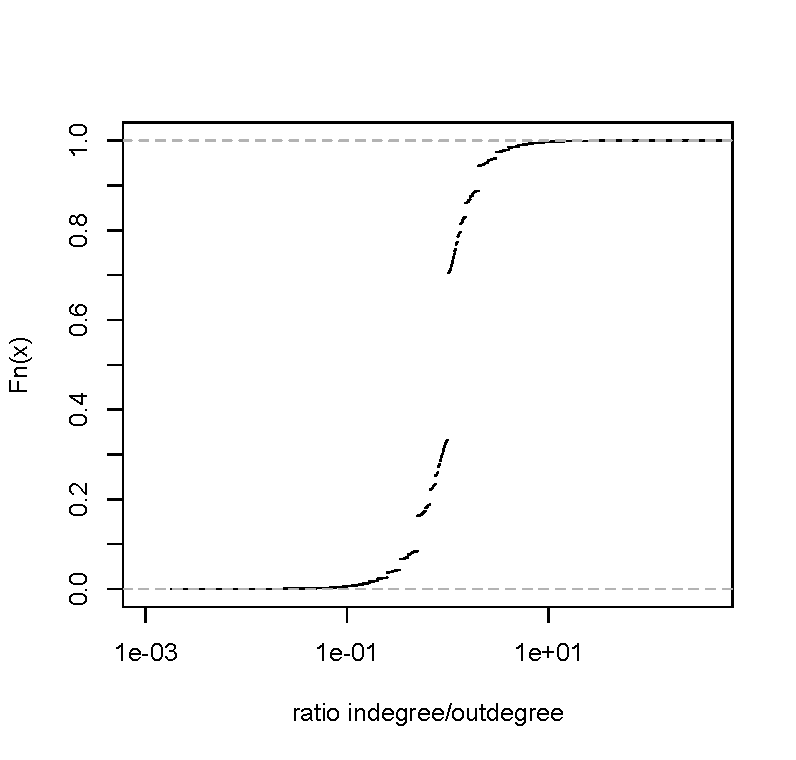
\includegraphics[scale=0.55]{images/inoutcorr.pdf}}
  \subfloat[]{\label{fig:knn} 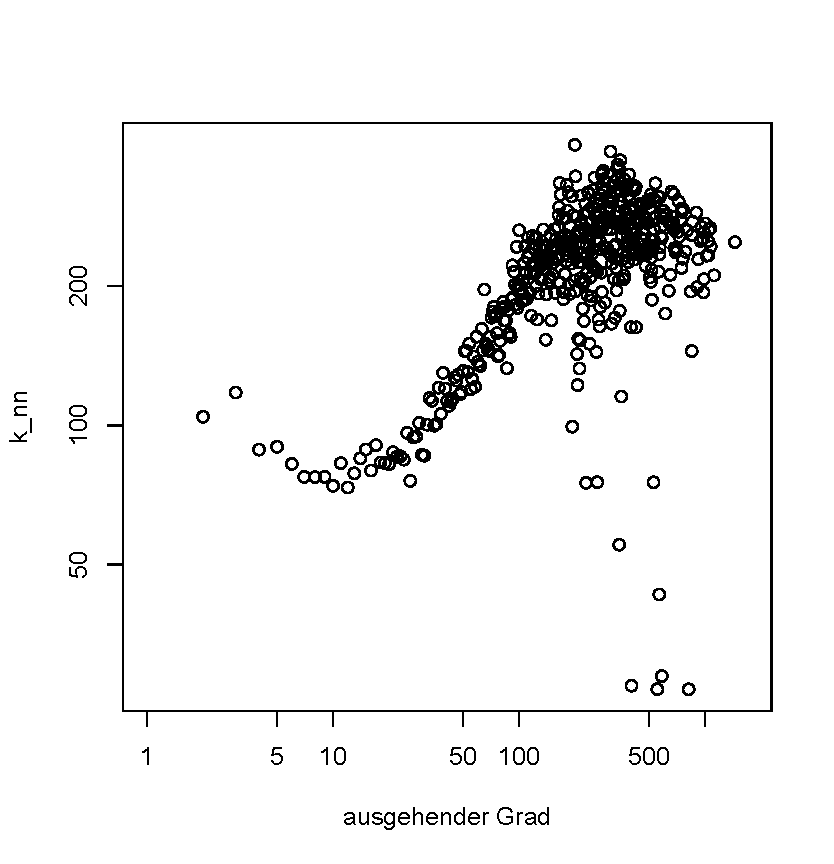
\includegraphics[scale=0.55]{images/knn.pdf}}
  \caption{Kumulative Verteilungsfunktion von $\frac{d^+(u)}{d^-(u)}$
    für alle Knoten $u$ in der MSCC
    \subref{fig:inoutcorr}. Verteilung von $k_{nn}$ über alle
    ausgehenden Grade \subref{fig:knn}.}
  \label{fig:degree-correlation}
\end{figure}

Für die Berechnung des Clustering-Koeffizienten wurde der eigentlich
gerichtete Graph als ungerichteter Graph betrachtet, da es keine
anerkannte Definition des Clustering-Koeffizienten für gerichtete
Graphen zu geben scheint. Diese Vorgehensweise scheint die in der
Literatur übliche zu sein. Selbstverständlich ist anzunehmen, dass
das Ergebnis verfälscht wird, wenn gerichtete Kanten als
ungerichtete Kanten betrachtet werden. Allerdings wurde bereits
gezeigt, dass ein erheblicher Anteil der Kanten symmetrisch ist, also
in beide Richtungen verläuft, und eine positive Korrelation zwischen
dem ausgehendem und dem eingehenden Grad von Knoten besteht. Die
Verf\"alschung des Ergebnisses
sollte sich also in Grenzen halten.

Der durchschnittliche Clustering-Koeffizient für die grösste
starke Zusammenhangskomponente beträgt $C = 0,460$. Das bedeutet,
dass \emph{im Durchschnitt} etwa die Hälfte der Nachbarn eines
Knoten wieder verbunden sind. Der Graph zeigt also ein erhebliches
Mass an Clustering. Zum Vergleich beträgt der Clustering-Koeffizient
für ein \emph{zufälliges} Netzwerk mit der gleichen Anzahl von
Knoten und Kanten $C = 0,00025$ und für ein zufälliges Netzwerk,
das ausserdem über die gleiche Sequenz von Graden verfügt, $C =
0,013$. In der größten starken Zusammenhangskomponente findet sich
also wesentlich mehr Clustering, als in einem zufällig entstandenen
Netzwerk zu erwarten wäre.

Newman und Park bemerken, dass ein hohes Mass an Clustering
charakteristisch für soziale Netzwerke ist und sie von vielen
nicht-sozialen Netzwerken unterscheidet \cite{PhysRevE.68.036122}. Als
möglichen Grund geben sie an, dass sich die Knoten in sozialen
Netzwerken üblicherweise in \emph{Communities} einteilen lassen,
also Gruppen von Knoten, die untereinander stärker vernetzt sind als
nach außen. Intuitiv ist nahe liegend, dass in einer solchen Community
die Wahrscheinlichkeit, dass zwei Nachbarn eines Knoten durch eine
Kante verbunden sind, hoch ist. In Abschnitt
\ref{sec:result-zusamm-und-comm} wird gezeigt, dass der vorliegende
Graph in der Tat über eine ausgepr\"agte Community-Struktur verfügt.

Der Durchschnitt aller Distanzen in der größten starken
Zusammenhangskomponente beträgt 12,14 (siehe auch Abbildung
\ref{fig:avg-pathlen} für die Verteilung der durchschnittlichen
Distanzen pro Knoten). Dieser Wert ist in Relation zur Anzahl der
Knoten im Netzwerk gering und zeigt, dass der Graph den
"`Small-World"'-Effekt aufweist, dass also Paare von Knoten mit
hoher Wahrscheinlichkeit durch einen Pfad von geringer Länge
verbunden sind. Dieser Effekt tritt in vielen untersuchten Netzwerken
auf und ist insbesondere typisch für soziale Netzwerke
\cite{newman:167}.

Interessant ist die geringe Distanz auch, weil die Teilnehmer des Web
of Trust aus verschiedensten Ländern und damit aus verschiedensten
geographischen Regionen stammen. Die übliche Prozedur für das
Signieren von Schlüsseln setzt ein direktes, d. h. räumliches
Treffen der teilnehmenden Personen voraus. Eine Interpretation der
geringen Distanz wäre, dass eine Anzahl von Teilnehmern geographisch
so mobil ist, dass sich Signierungen an weit auseinander liegenden
Orten ergeben, die für die Verbindungen zwischen geographisch
eigentlich weit entfernten Bereichen im Netzwerk sorgen. Allerdings
wurde hier nur der Durchschnitt der Distanzen betrachtet. Es kann
nicht ausgeschlossen werden, dass sich der niedrige Durchschnitt für
die einzelnen Knoten nur ergibt, weil die Knoten aus dem eigenen Land
bzw. der eigenen geographischen Region auch im Netzwerk sehr nahe
liegen. In Abschnitt \ref{sec:result-zusamm-und-comm} wird gezeigt,
dass sich die meisten Communities anhand von Top-Level-Domains einem
Land oder Sprachraum zuordnen lassen. Interessant wäre an dieser
Stelle eine Untersuchung, inwiefern sich die geographische Distanz der
Länder auch in der Distanz im Netzwerk der entsprechenden
Communities wiederspiegelt.

\subsubsection{Verteilung der Grade, Skalenfreiheit}
\label{sec:verteilung-der-grade}

\begin{figure}[th!]
  \centering
  \subfloat[]{\label{fig:indeg-dist} 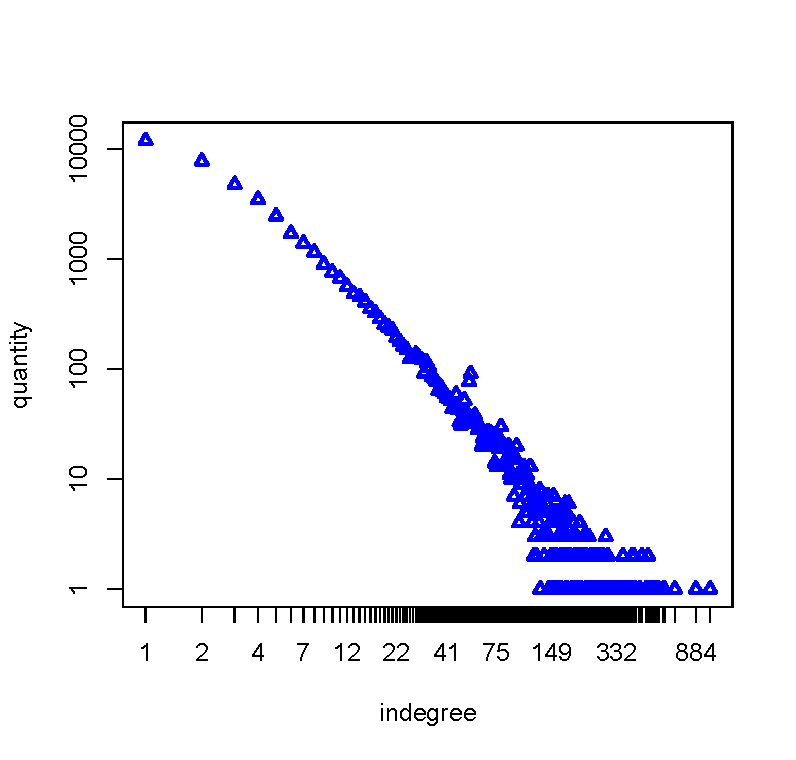
\includegraphics[scale=0.42]{images/indegree-dist.pdf}}
  \subfloat[]{\label{fig:outdeg-dist} 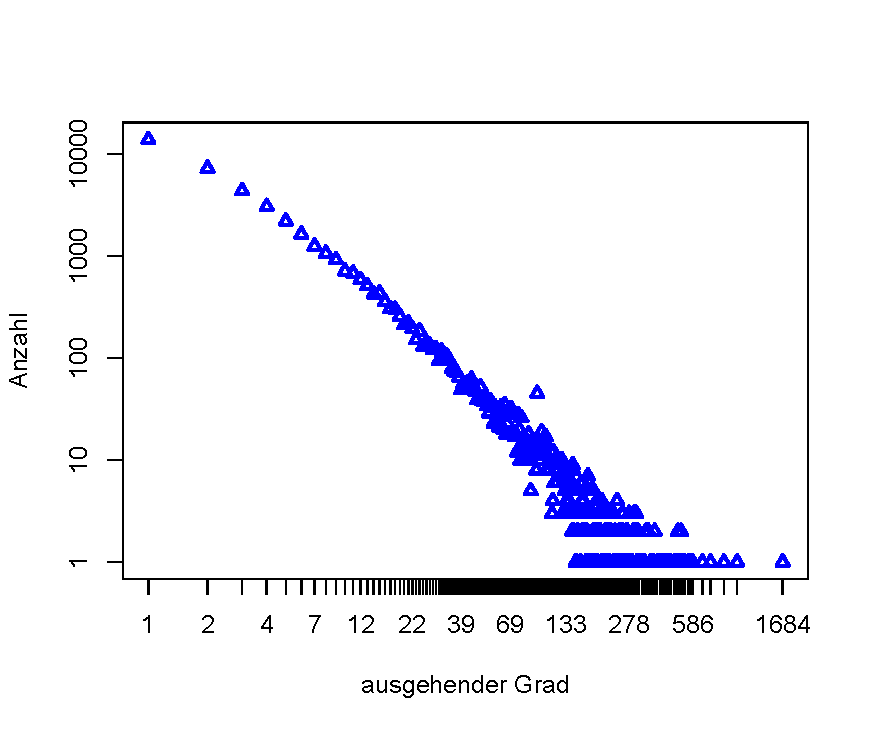
\includegraphics[scale=0.42]{images/outdegree-dist.pdf}}
  \caption{Verteilung der eingehenden \subref{fig:indeg-dist} und
    ausgehenden \subref{fig:outdeg-dist} Knotengrade in der grö{\ss}ten
    starken Zusammenhangskomponente.}
  \label{fig:degree-dist}
\end{figure}

Der durchschnittliche ausgehende Grad (und damit auch der
durchschnittliche eingehende Grad) beträgt 9,29. Allerdings zeigen
Abbildung \ref{fig:indeg-dist} und \ref{fig:outdeg-dist}, dass dieser
Durchschnitt auf höchst ungleichmäßige Weise zustande kommt. Während
eine Mehrheit der Knoten einen sehr kleinen ein- bzw. ausgehenden Grad
hat, existiert eine signifikante Anzahl von Knoten, deren Grad
deutlich über dem Durchschnitt liegt. Dieses Verhalten scheint konsistent
mit einer Power-Law-Verteilung der Grade und die in etwa geraden
Linien im doppelt logarithmischen Plot der Verteilungen legen dies
zusätzlich nahe. Allerdings wird in \cite{Clauset2009} argumentiert,
dass ein "`Nachweis"' einer Power-Law-Verteilung und insbesondere die
Berechnung des Power-Law-Koeffizienten etwa mit linearer Regression
auf einem doppelt logarithmischen Plot (vorgeschlagen etwa bei
\cite{Brinkmeier2004}) zu stark verfälschten Ergebnissen führen
kann. Stattdessen wird hier die von Clauset et al. vorgeschlagene
Vorgehensweise benutzt, die beste Power-Law-Anpassung mittels der
Maximum-Likelihood-Methode zu berechnen. Damit ergibt sich für die
Verteilung der ein- bzw. ausgehenden Grade ein Power-Law-Koeffizient
von 2,35 bzw. 2,29. Allerdings ergibt die Überprüfung der Qualität der
Anpassung mittels des Kolmogorov-Smirnov-Tests Werte, die mit $p =
0,012$ und $p = 0,011$ deutlich unter dem in \cite{Clauset2009}
empfohlenen Schwellwert von $p=0,1$ liegen und damit ein Power-Law als
plausible Hypothese für die Verteilung ausschließen.


Es handelt sich bei dem vorliegenden Netzwerk also nicht um ein
skalenfreies Netzwerk im engeren Sinne. Es stellt sich allerdings die
Frage, ob das überhaupt relevant ist. Zum einen zeigt die Verteilung
der Grade Merkmale, die mit charakteristischen Merkmalen einer
Power-Law-Verteilung übereinstimmen, nämlich die hohe
Variabilität der Grade und insbesondere die Anwesenheit einer
signifikanten Anzahl von Knoten mit hohem Grad. Die Verteilung
\emph{ähnelt} also immerhin einer Power-Law-Verteilung. Eine
zentrale Rolle bei den Eigenschaften, die skalenfreien Netzwerken
zugeschrieben werden, spielt die Existenz eines Kerns bestehend aus
untereinander verbundenen, stark vernetzten "`Hubs"'. Knoten mit niedrigem Grad sind primär mit diesen Hubs
verbunden. Dieser Kern ist essentiell  f\"ur den Zusammenhang des
Netzwerkes und sorgt für
geringe Distanzen. Allerdings haben Li et al. \cite{Li2005} gezeigt,
dass die Existenz einer Power-Law-Verteilung nicht ausreicht, um die
Existenz von Hubs nachzuweisen. Es existieren Netzwerke, die zwar eine
Power-Law-Verteilung der Grade haben, bei denen die Knoten mit hohem
Grad aber eher an der \emph{Peripherie} liegen und keine zentrale
Rolle im Sinne von Hubs übernehmen.  Hubs ergeben sich erst dann,
wenn Knoten mit hohem Grad primär mit Knoten vernetzt sind, die
wiederum einen hohen Grad haben. Eine tatsächliche
Power-Law-Verteilung ist für die Existenz einer Hub-Struktur nicht
notwendig, es reicht als notwendiges Kriterium bereits eine Verteilung
mit hoher Variabilität (ebd.). Eine solche ist hier vorhanden.

Um zu überprüfen, ob die gut vernetzten Knoten tatsächlich als
Hubs fungieren, wurde zunächst die Korrelationsfunktion $k_{nn}$
berechnet. Diese verbindet für gerichtete Graphen einen Grad $d$ mit
dem Durchschnitt des Grads der Nachbarn der Knoten, die diesen Grad
$d$ haben. Sie misst also, wie hoch der Grad von Knoten ist, die mit
Knoten vom Grad $d$ verbunden sind. Abbildung \ref{fig:knn} zeigt die
Verteilung von $k_{nn}$ über alle Grade $d$. Aus der ansteigenden
Kurve für ansteigende Grade kann geschlossen werden, dass Knoten mit
hohem Grad dazu tendieren, zu anderen Knoten mit hohem Grad verbunden
zu sein. Diese Knoten scheinen also in der Tat einen \emph{Kern} des
Netzwerkes zu bilden. Um dies zu untermauern, wurde zusätzlich noch
der Assortativity-Koeffizient $r$ \cite{PhysRevLett.89.208701}
berechnet. Ein positiver Wert von $r$ bedeutet, dass eine positive
Korrelation zwischen den Graden der Knoten besteht. Im
gegensätzlichen Fall einer negativen Korrelation ist $r$ negativ. Es
ergibt sich ein Wert $r = 0,113$. Aus diesem positiven Wert folgt also
ebenfalls, dass Knoten tendenziell mit Knoten verbunden sind, die
einen ähnlichen Grad haben. Der $r$-Wert ähnelt den Werten, die
für andere soziale Netzwerke berechnet wurden \cite{newman:167}.

\subsection{Robustheit}
\label{sec:robustheit}

\begin{figure}[ht!]
  \centering
  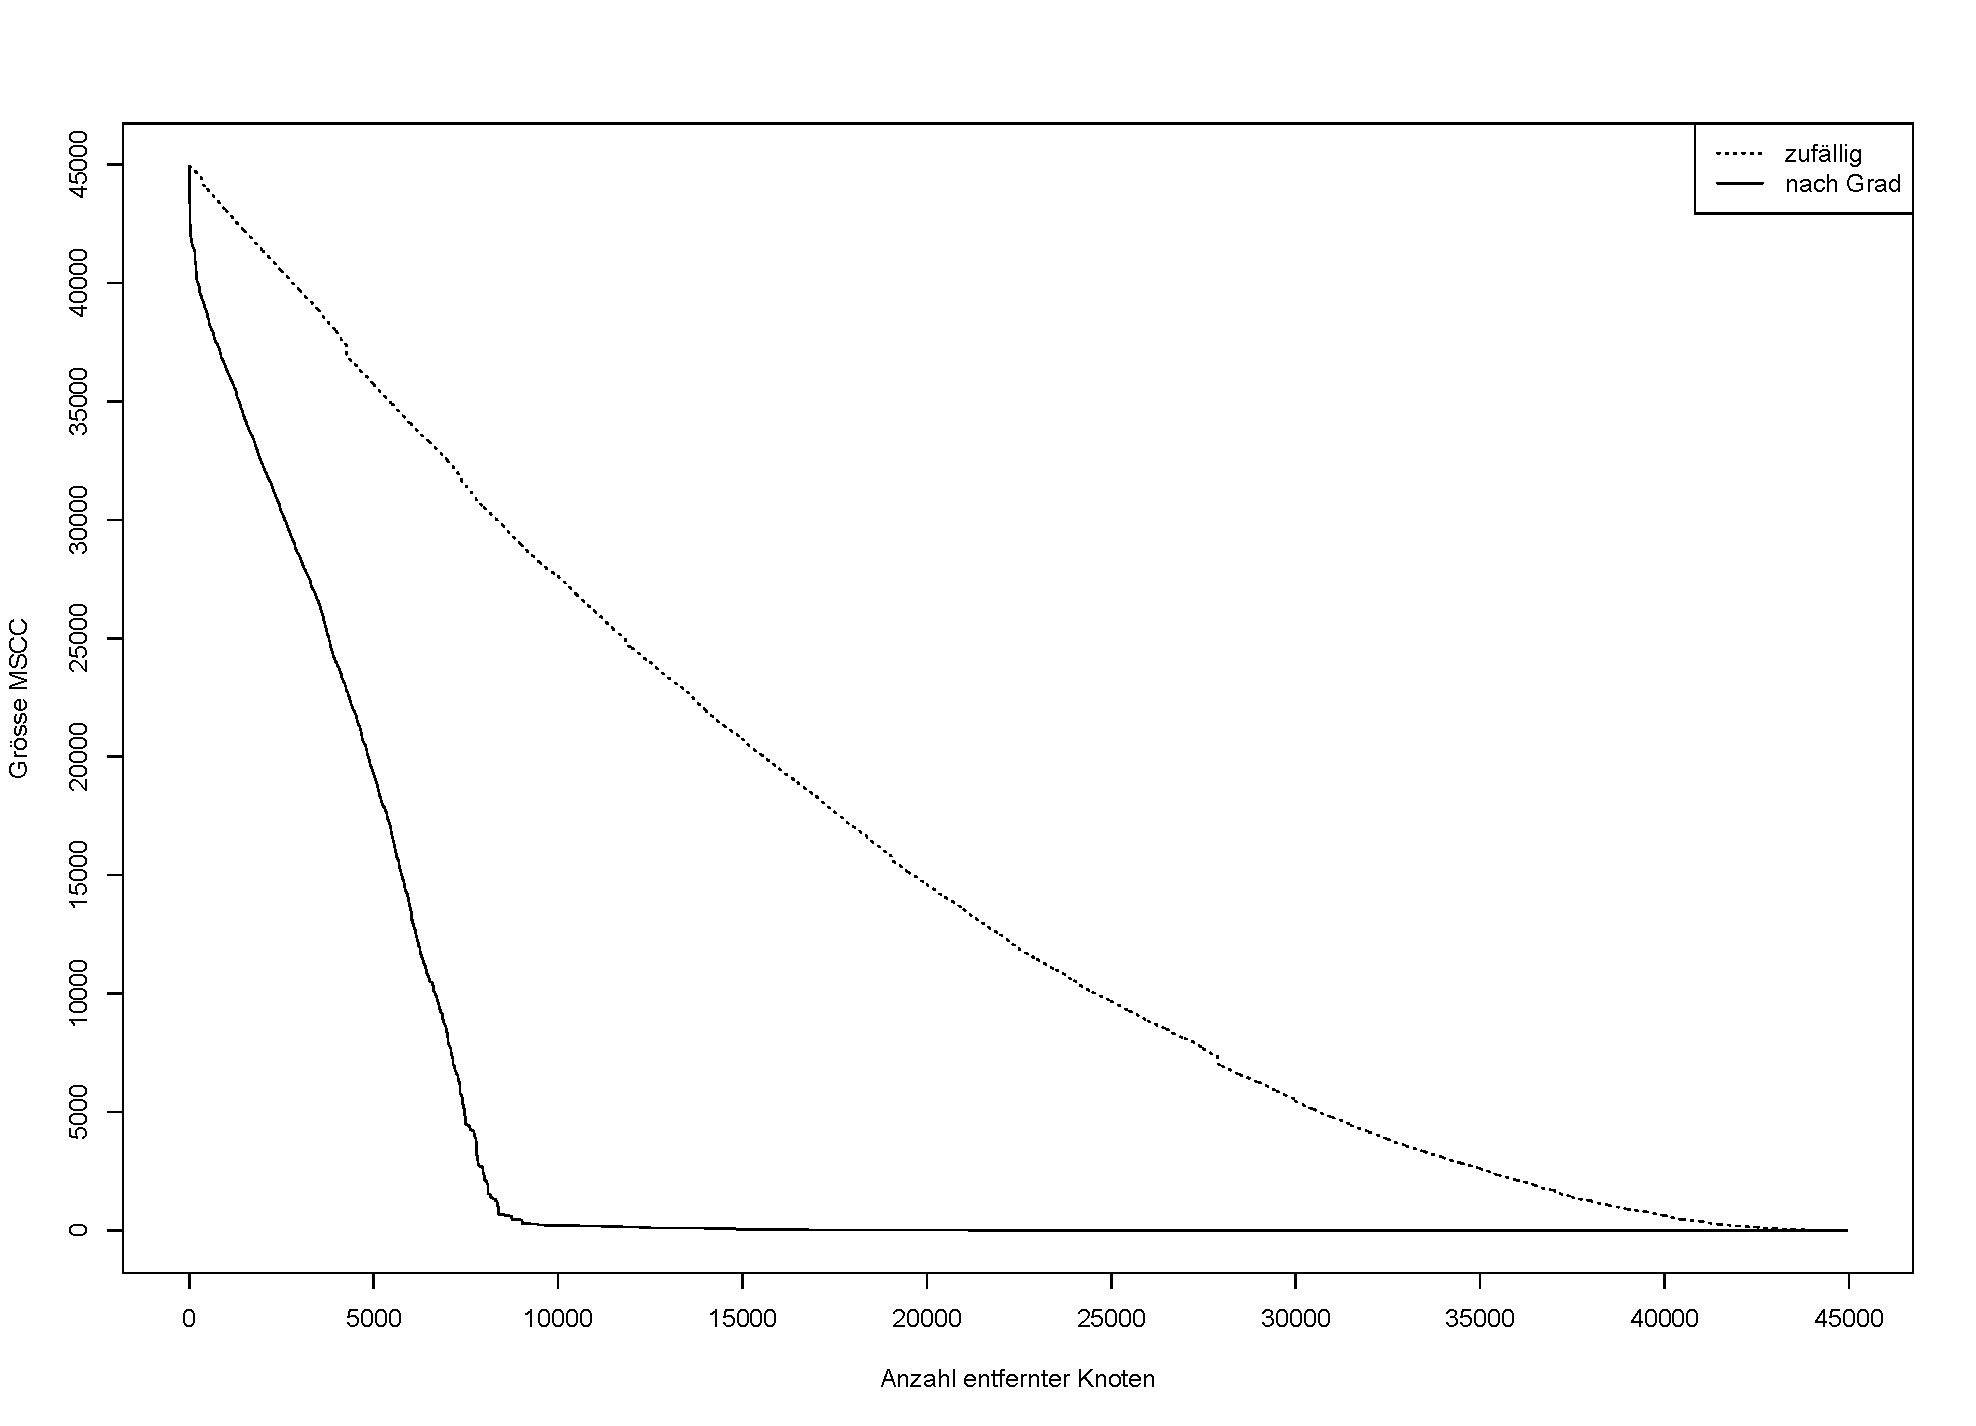
\includegraphics[scale=0.45]{images/without.pdf}
  \caption{Entwicklung der Größe der größten starken
    Zusammenhangskomponente, wenn Knoten zufällig oder nach absteigender
    Größe entfernt werden}
  \label{fig:without}
\end{figure}

In diesem Zusammenhang stellt sich auch die Frage nach der
\emph{Robustheit} des Netzwerkes.  Eine Eigenschaft, die skalenfreien
Netzwerken üblicherweise zugeschrieben wird, ist eine
charakteristische Reaktion auf das Entfernen von Knoten: Während die
Entfernung zufällig ausgewählter Knoten kaum Schaden anrichtet,
reagiert das Netzwerk sehr verwundbar auf die Entfernung von Knoten,
die sehr gut vernetzt sind. Schon die Entfernung weniger sehr gut
vernetzter Knoten führt dazu, dass das Netzwerk
zerfällt. Dieses Verhalten wird damit erkl\"art, dass der Zusammenhang des
Netzwerks fast ausschlie{\ss}lich durch die kleine Gruppe sehr stark
vernetzter Hubs bestimmt wird \cite{Albert2000}.

Dieser Unterschied kann aufgefasst werden als der Unterschied zwischen
einem gerichteten \emph{Angriff} und einer zufälligen
\emph{Schädigung}. Ein Angreifer mit der Intention, das Netz an sich
zu schädigen, wird solche Knoten auswählen, deren Entfernung einen
möglichst großen Effekt hat. Demgegenüber kann angenommen werden,
dass die Wahrscheinlichkeit einer zufälligen Schädigung in etwa
gleich verteilt über alle Schlüssel ist. Ein Angreifer könnte
beispielsweise versuchen, Knoten zu entfernen, indem er den
Schlüssel an sich kompromittiert oder den Zugriff auf das
Schlüsselmaterial unmöglich macht, so dass der Schlüssel
widerrufen werden muss. Demgegenüber können Schlüssel auf
"`normalem"' Wege aus dem Netz verschwinden, wenn sie ablaufen oder
beispielsweise aufgrund des Verlusts der Passphrase widerrufen werden
müssen.

Eine offensichtliche Metrik für die Wichtigkeit eines Knotens und
damit eine Strategie für die Auswahl des Zielknotens ist der
Knotengrad. Je höher der Grad eines Knotens, desto wichtiger ist er
potentiell für das Netzwerk. Um die Robustheit unter dieser
Auswahlstrategie zu testen, wurden aus der größten starken
Zusammenhangskomponente sukzessive Knoten in der Reihenfolge
absteigender ausgehender Grade bzw. in einer zufälligen Reihenfolge
entfernt. Abbildung \ref{fig:without} zeigt die Entwicklung der Größe
der größten Komponente, wenn mehr und mehr Knoten entfernt werden. Bei
der Entfernung zufällig ausgewählter Knoten ist das Netzwerk
ausgesprochen stabil. Die größte Komponente schrumpft fast im gleichen
Ausma{\ss}, wie Knoten entfernt werden, woraus geschlossen werden kann,
dass nur einzelne Knoten oder sehr kleine Gruppen abgetrennt werden. Dieses Ergebnis ist nicht
überraschend. Da ein hoher Anteil der Knoten einen sehr niedrigen Grad
hat, ist bei zufälliger Auswahl die Chance, einen solchen Knoten zu
treffen, hoch. Das Verschwinden von Schlüsseln durch die
\"Uberschreitung des Ablaufdatums ist ein
normaler und häufiger Prozess. So verfügen etwa 5.700 Schlüssel in der
größten starken Zusammenhangskomponente über ein Ablaufdatum, werden
also irgendwann aus dem Netz verschwinden. Dieser Fall richtet also
kaum globalen Schaden im Netzwerk an.

Abbildung \ref{fig:without} zeigt ebenfalls, dass die Entfernung von
Knoten geordnet nach absteigendem ausgehendem Grad die Gr\"o{\ss}e der
gr\"o{\ss}ten starken Zusammenhangskomponente deutlich schneller reduziert als im
Fall der zuf\"alligen Reihenfolge. Dies ist nicht verwunderlich, da
bei der geordneten Reihenfolge am Anfang mit jedem Knoten im
Durchschnitt eine sehr viel gr\"o{\ss}ere Anzahl von Kanten
entfernt wird. Da das Netzwerk eine sehr gro{\ss}e Anzahl von Knoten mit
sehr niedrigem Grad enth\"alt, ist die Wahrscheinlichkeit hoch, dass
eine Reihe dieser Kanten solche schlecht vernetzten Knoten
vollst\"andig abtrennt.

Andererseits ist die Abnahme der Gr\"o{\ss}e der MSCC zu langsam, als
dass von einem rapiden Zerfall gesprochen werden k\"onnte. Die
Entfernung der 240 Knoten mit den h\"ochsten Graden -- dies entspricht
der Entfernung aller Knoten mit einem ausgehenden Grad von mindestens
160 -- reduziert die
Gr\"o{\ss}e der MSCC auf 40.000 Knoten. Auch wenn damit eine
signifikante Anzahl von Knoten abgetrennt wird, wird das Netzwerk als
Solches damit noch lange nicht fundamental fragmentiert. Selbst die
Entfernung von 5000 Knoten (d.h. Knoten mit einem Grad von mindestens
18) l\"a{\ss}t noch eine gr\"o{\ss}te starke Zusammenhangskomponente von
etwa 20.000 Knoten \"ubrig.

Es zeigt sich, dass die am besten vernetzten Knoten nicht so zentral
f\"ur den Zusammenhang des Netzwerkes sind, dass schon die Entfernung
einer kleinen Anzahl dieser Knoten zu einer rapiden Fragmentierung
f\"uhrt. Die Fragmentierung verl\"auft deutlich langsamer als in der
Literatur f\"ur untersuchte "`skalenfreie"' Netzwerke angegeben
(beispielsweise bei \cite{Albert2000}). Es scheint damit keine
Hub-Struktur im Sinne der Literatur zu "`skalenfreien"' Netzwerken
vorzuliegen. 

Das Netzwerk scheint also selbst gegen\"uber einer sehr gro{\ss}
angelegten Attacke recht robust zu sein. Die Möglichkeiten eines realistischen Angreifers dürften
sich eher im Entfernen einzelner Knoten erschöpfen, so dass der zu
erwartende Schaden gering ist. 

Angemerkt werden muss aber , dass neben der Größe der Komponente auch
eine Betrachtung der Entwicklung der Distanzen in der Komponente
sinnvoll wäre. Dass die Größe der Komponente sich im Fall
zufälliger Reihenfolge sehr stabil und im Fall der geordneten
Reihenfolge recht stabil verhält, muss nicht bedeuten, dass
sich die durchschnittlichen Distanzen nicht deutlich
vergrößern. Vergrößern sich die Distanzen und verlängern sich
damit die nötigen Signaturketten, so sinkt die Nützlichkeit des
Netzwerkes (siehe Abschnitt \ref{sec:nutzlichkeit}). Für die
Entfernung von Knoten anhand des Grades wird
erwartet, dass sich die
Distanzen schon durch die Entfernung weniger Knoten merklich
erhöhen. Aufgrund des notwendigen Rechenaufwandes konnte dies im
Rahmen dieser Arbeit aber nicht \"uberpr\"uft werden.

Der Grad eines Knotens ist nicht unbedingt das geeignetste Ma{\ss} für
die globale "`Wichtigkeit"' des Knotens. Durch eine Konzentration auf
\emph{zentrale} Knoten, also etwa solche mit einer hohen Betweeness
Centrality, lässt sich möglicherweise mehr Schaden anrichten. Dies
lässt sich am Beispiel von Certificate Authorities im Web of Trust
illustrieren: CA-Schlüssel haben zwar üblicherweise einen hohen
ausgehenden Grad, haben also viele Schlüssel signiert und damit
relativ kurze Wege zu vielen Schlüsseln. Allerdings haben sie
\"ublicherweise gleichzeitig einen niedrigeren eingehenden Grad, weil ein CA-Schlüssel
üblicherweise nicht mit einer Person direkt verbunden ist, und damit
das übliche Verifizieren der Identität wenig Sinn macht. Damit tauchen
CA-Schlüssel nur auf relativ wenigen kürzesten Pfaden auf, da sie
selbst eher schlecht erreichbar sind. Ihre Entfernung richtet also --
zumindest in Bezug auf die Distanzen -- einen relativ geringen Schaden
an.

\subsection{Nützlichkeit}
\label{sec:nutzlichkeit}
Dieser Abschnitt betrachtet die Nützlichkeit des Netzwerkes für
seinen eigentlichen Zweck, die Verifizierung von Schlüsseln. Diese
Nützlichkeit ist dann hoch, wenn für viele Knoten eine hohe Zahl
von Knoten potentiell verifizierbar ist.

Eine Mindestvoraussetzung für die Verifizierung eines Schlüssels
ist, dass eine Signaturkette zu diesem Schlüssel aufgebaut werden
kann, dass also der Knoten im Graph erreicht werden kann. Dies ist in
einer starken Zusammenhangskomponente der Fall, da laut Definition ein
Pfad von jedem Knoten zu jedem anderem Knoten besteht. Allerdings ist
die Erreichbarkeit an sich hier nicht von Bedeutung. Vielmehr muss die
Erreichbarkeit unter den Beschränkungen des
PGP/GnuPG-Vertrauensmodells (siehe Abschnitt
\ref{sec:das-gnupg-vertrauensmodell}) betrachtet werden. Hier gilt
insbesondere die Einschränkung, dass Signaturketten in der
Standardeinstellung maximal die Länge 5 haben
dürfen. Selbstverständlich bedeutet das Vorhandensein einer
Signaturkette von hinreichend geringer Länge noch nicht, dass ein
Schlüssel tatsächlich verifizierbar ist. Zusätzlich muss noch
jedem Glied dieser Kette \emph{vertraut} werden. Wird Personen nur
\emph{geringfügig} vertraut, sind zusätzlich noch weitere
redundante Signaturen nötig. Da diese Vertrauensinformationen aber
nicht öffentlich verfügbar sind, wird hier als obere Grenze für
die Anzahl verifizierbarer Schlüssel nur die maximale Pfadlänge
verwendet.

Die größte Komponente enthält eine erhebliche Anzahl von Knoten
mit einem ausgehenden Knotengrad von 1. Ein solch niedriger Grad
stellt eine erhebliche Einschränkung für die Benutzbarkeit dieses
Schlüssels für die Verifizierung von anderen Schlüsseln dar. Da
ein Schlüssel $A$ mit ausgehendem Grad 1 nur einen Schlüssel $B$
signiert hat, gibt es auch nur genau einen Schlüssel, über den
eine Signaturkette aufgebaut werden kann. Natürlich wird dadurch die
Menge der insgesamt erreichbaren Knoten stark eingeschränkt. Außerdem
aber existiert damit keine Redundanz. Der Besitzer des Schlüssels
$A$ muss dem Besitzer des Schlüssels $B$ vertrauen, wenn er irgendeine 
Signaturkette benutzen will. $B$ stellt einen \emph{Single point
  of failure} dar, da $A$ vom Netz getrennt wird, wenn $B$ etwa
abläuft oder zurückgezogen wird. Äquivalent ist die
Verifizierbarkeit eines Knotens $A$ stark eingeschränkt, wenn er
einen eingehenden Grad von 1 hat und nur von einem einzigen
Schlüssel $B$ signiert wurde. Für die Verifizierung von $A$ muss
zwingend dem Besitzer von $B$ vertraut werden. Ist $B$ nicht mehr
benutzbar, wird $A$ vom Netz getrennt.

\begin{figure}[th!]
  \centering
  \subfloat[]{\label{fig:avg-pathlen}\includegraphics[scale=0.3]{images/pathlen-dist.pdf}}
  \subfloat[]{\label{fig:eccentricity}\includegraphics[scale=0.3]{images/ecc-dist.pdf}}
  \caption{Verteilung der (gerundeten) durchschnittlichen Distanzen 
    \subref{fig:avg-pathlen} und der Eccentricity
    \subref{fig:eccentricity} in der größten starken Zusammenhangskomponente}
  \label{fig:pathlen-dist}
\end{figure}

Aus Abbildung \ref{fig:eccentricity} ist ersichtlich, dass die
Eccentricity, also die \emph{maximale} Distanz eines Knotens zu
einem anderen Knoten, zwischen dem Minimum 16 (dem \emph{Radius}
des Graphen) und dem Maximum 36 (dem \emph{Durchmesser} des Graphen)
liegt. Für die meisten Knoten liegt sie bei 26 bis 31. Damit wird
die maximale Pfadlänge deutlich überschritten. Für alle Knoten
gilt also, dass die am weitesten entfernten Knoten grundsätzlich
nicht erreichbar sind. Aber auch schon die \emph{durchschnittliche}
Distanz (Abbildung \ref{fig:pathlen-dist}) ist für eine erhebliche
Anzahl von Knoten größer als die maximal erlaubte Länge. Klar ist
also, dass für die Mehrzahl der Knoten längst nicht alle Knoten
unter der Beschränkung der Pfadlänge erreichbar sind.

Die Größe der 5-Nachbarschaft eines Knotens gibt die Anzahl der
Knoten an, die unter dieser Beschränkung erreichbar sind. Allerdings
macht es Sinn, nicht nur die 5-Nachbarschaft, sondern auch die
$n$-Nachbarschaften für $n=2,\dots,4$, also kürzere
Signaturketten, zu betrachten. Da jedem einzelnen Glied einer
Signaturkette vertraut werden muss, steigt mit der Länge der Kette
auch die Wahrscheinlichkeit, dass dieses Vertrauen eben nicht in alle
Glieder vorhanden ist. Da das Web of Trust ein soziales Netzwerk
darstellt, kann angenommen werden, dass im Allgemeinen mit der
Entfernung zu einem Knoten im Graph auch die soziale und geographische
Entfernung zu der entsprechenden Person steigt. Damit sinkt auch die
Wahrscheinlichkeit, dass weiter entfernten Personen aufgrund von
persönlicher Bekanntschaft vertraut werden kann. Dass einer Person,
deren Schlüssel selbst signiert wurde, vertraut wird, ist
wahrscheinlicher als dass einer Person vertraut wird, deren
Schlüssel nicht selbst signiert wurde. Es scheint also plausibel, dass
die Wahrscheinlichkeit f\"ur die Benutzbarkeit einer Signaturkette
sinkt, je l\"anger diese wird. 

\begin{figure}[th!]
  \centering
  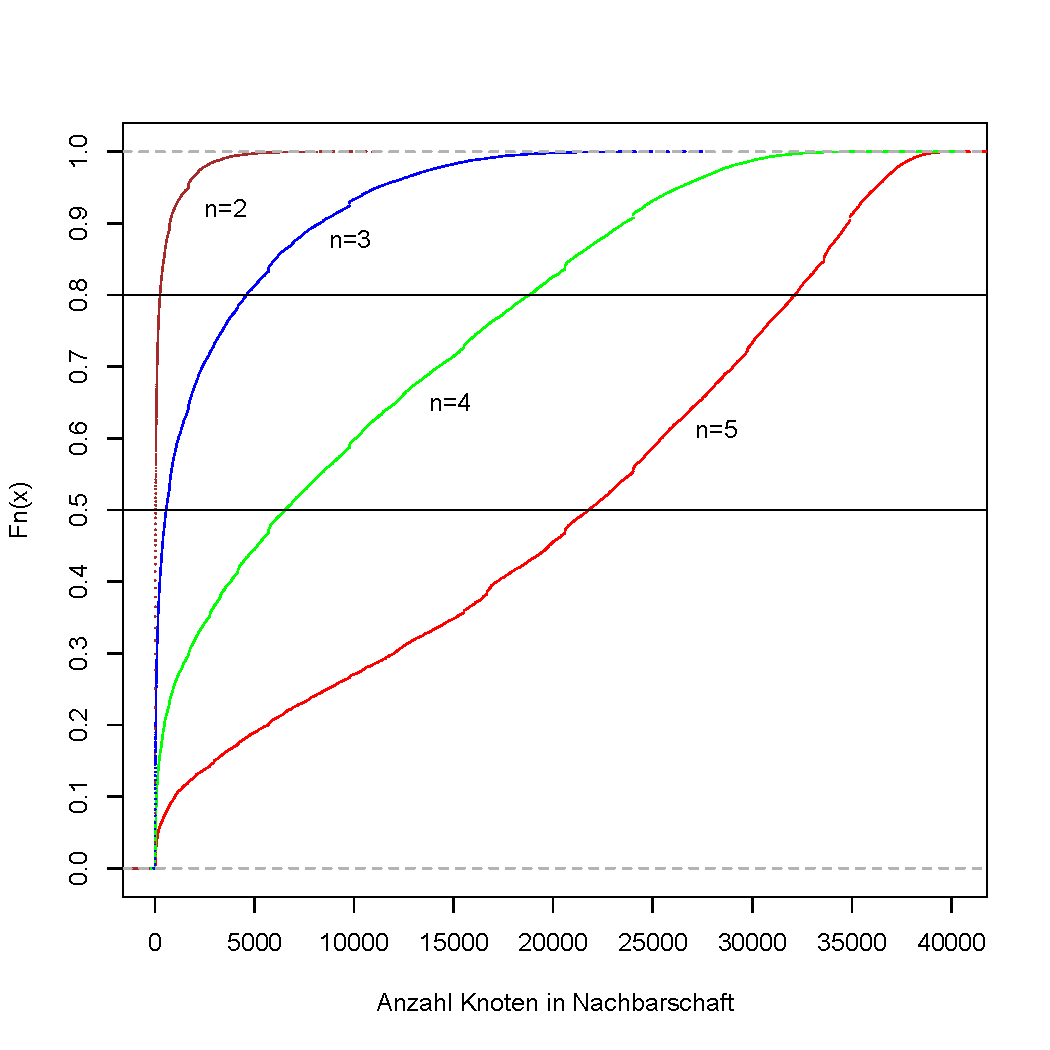
\includegraphics[scale=0.6]{images/neighbourhood-cdf.pdf}
  \caption{Kumulative Verteilungsfunktion der Nachbarschaftsgrö{\ss}en
    in der größten starken Zusammenhangskomponente}
  \label{fig:neighbourhood-cdf}
\end{figure}

Abbildung \ref{fig:neighbourhood-cdf} zeigt die kumulative
Verteilungsfunktion der Größe der Nachbarschaften. Auffällig
ist hier zunächst das steile Wachstum der Kurve für die
2-Nachbarschaft, woraus geschlossen werden kann, dass diese
Nachbarschaft für fast alle Knoten sehr klein ist. In der Tat liegt
das 2. Quartil bei 30 und das 3. Quartil bei 160. Für die Mehrzahl
der Schlüssel ist also die Menge der Schlüssel, für deren
Verifizierung nur einer Person voll vertraut werden muss, sehr
gering. Immerhin steigt die Größe der Nachbarschaften mit
wachsender Distanz deutlich: Für $n=3$ liegt das 3. Quartil bereits
bei 3.371. Für $n=4$ und $n=5$ beträgt es 16.340 bzw. 30.530. Mittels
längerer Signaturketten kann also die Mehrzahl der Teilnehmer einen
signifikanten Anteil der in der größten Zusammenhangskomponente
vorhandenen Schlüssel \emph{potentiell}
erreichen. Interessanterweise liegt das Maximum der
Größe der Nachbarschaften für $n=5$ bei nur 40.180. Nicht einmal für
die am besten vernetzten Schlüssel sind also alle Schlüssel mit
beschränkter Kettenlänge erreichbar.

Wie bereits erwähnt, enthält die größte Zusammenhangskomponente
die Schlüssel mehrerer zentraler Certificate
Authorities. Interessant ist eine Abschätzung, wie sehr das
eigentlich dezentrale Web of Trust auf diese zentralen Komponenten
aufbaut. Um dies festzustellen wurden die Schlüssel der größeren
Certificate Authorities (siehe Abschnitt \ref{sec:sozi-komp-des}) aus
der größten Komponente entfernt. Diese CA-Schlüssel haben
zusammen in dieser Komponente 4.256 Schlüssel signiert. Nach der
Entfernung der CA-Schlüssel zerfiel die größte Komponente in eine
Reihe von starken Zusammenhangskomponenten: Eine größte Komponente
mit 42.455 Schlüsseln und 1.058 sehr kleine Komponenten. Daraus ergibt
sich, dass die CA-Schlüssel die größte Komponente zwar nicht
fundamental zusammenhalten. Für immerhin 2.497 Schlüssel in der
größten Zusammenhangskomponente ist aber das Vorhandensein und die
Benutzung der CA-Schlüssel entscheidend, da sie andernfalls nicht
erreichbar sind.

\section{Communities}
\label{sec:result-zusamm-und-comm}

\subsection{Ergebnisse für den gerichteten Graphen}
\label{sec:ergebnisse-fur-den}

Die Zerlegung des gerichteten Graphen mit dem Algorithmus von Rosval
et al. lieferte keine verwertbaren Ergebnisse. Zwar wurde eine
Zerlegung in 2869 Partitionen berechnet. Allerdings gilt für die
große Mehrzahl dieser Knotenmengen, dass der durch sie induzierte
Teilgraph überhaupt keine Kanten hat. Nur für ca. 160 Partitionen
hat der jeweils induzierte Teilgraph Kanten, in allen Fällen
allerdings sehr wenige (zwischen 1 und 104 für eine Partition der
Größe 682). Dass die Knoten einer Partition in allen Fällen so
gut wie keine interne Vernetzung haben und damit der Definition von
Communities absolut nicht entsprechen, ist ein klarer Hinweis, dass
die berechnete Zerlegung die tatsächliche modulare Struktur des
Graphen nicht sinnvoll wiedergibt. Dass der Graph in der Tat eine
ausgeprägte modulare Struktur hat, zeigen die anhand des
ungerichteten Graphen berechneten Zerlegungen, die auch unter
inhaltlichen Gesichtspunkten Sinn ergeben.  Die berechnete Zerlegung mit etlichen
großen Partitionen ohne interne Vernetzung ist in keinem Fall ein
sinnvolles Ergebnis eines Community-Algorithmus und spricht daher
für eine fehlerhafte Berechnung. Ob diese allerdings auf Fehler in
der verwendeten Implementierung der Autoren
\footnote{http://www.tp.umu.se/\~{}rosvall/code.html} oder auf Fehler im
Algorithmus zurückgeht, ist nicht bekannt.

\subsection{Ergebnisse für den ungerichteten Graphen}
\label{sec:ergebnisse-fur-den-1}

Für die restlichen Methoden wurde der Graph auf einen ungerichteten
Graphen reduziert. Dazu wurde jede einzelne gerichtete Kante in eine
ungerichtete Kante umgewandelt. Aus dem gerichteten Graphen mit 446.326
Kanten ergab sich so ein ungerichteter Graph mit 295.425 Kanten.

Für die COPRA-Berechnung wurden -- wie in \cite{Gregory2010}
vorgeschlagen -- Berechnungen mit unterschiedlichen Werten $v$
durchgeführt, um den "`besten"' Wert im Sinne der Modularity zu
ermitteln. Dabei ergaben sich mit steigender maximaler Überlappung
$v$ nur bis $v\le 3$ steigende Modularity-Werte, darüber hinaus
fielen sie kontinuierlich ab. Deshalb wurde die Berechnung mit $v=3$
verwendet. Die dort berechneten Modularity-Werte hatten eine geringe
Standardabweichung von 0,003. Dieses Ergebnis kommt unerwartet. In
\cite{Gregory2010} ergaben sich für ein PGP-Web-of-Trust-Netzwerk
mit 10.680 Knoten bis zu $v=9$ ansteigende Modularity-Werte. Das
(lokale) Maximum bei geringem $v$ für das hier verwendete Netzwerk
könnte darauf hinweisen, dass seine Community-Struktur keine
signifikante Überlappung aufweist. Ein weiterer Hinweis darauf ist,
dass die Einführung der Überlappung mit $v=3$ gegenüber der
nicht überlappenden Berechnung mit $v=1$ für die Modularity
(Tabelle \ref{tab:mod-result}) keinen signifikanten Anstieg
brachte. Auch die Zuordnung zu Gruppen bzw. Keysigning-Parties
(Tabelle \ref{tab:assign}) und die Verteilung der Größe der
Communities (Abbildungen \ref{fig:comsize-copra} und
\ref{fig:comsize-copra1}) ähneln sich weitgehend. Alternativ
könnte dieses Ergebnis allerdings auch in einem nicht-optimalen
Verhalten des Algorithmus begründet liegen.

\begin{figure}[th!]
  \centering
  \subfloat[]{\label{fig:comsize-copra1} 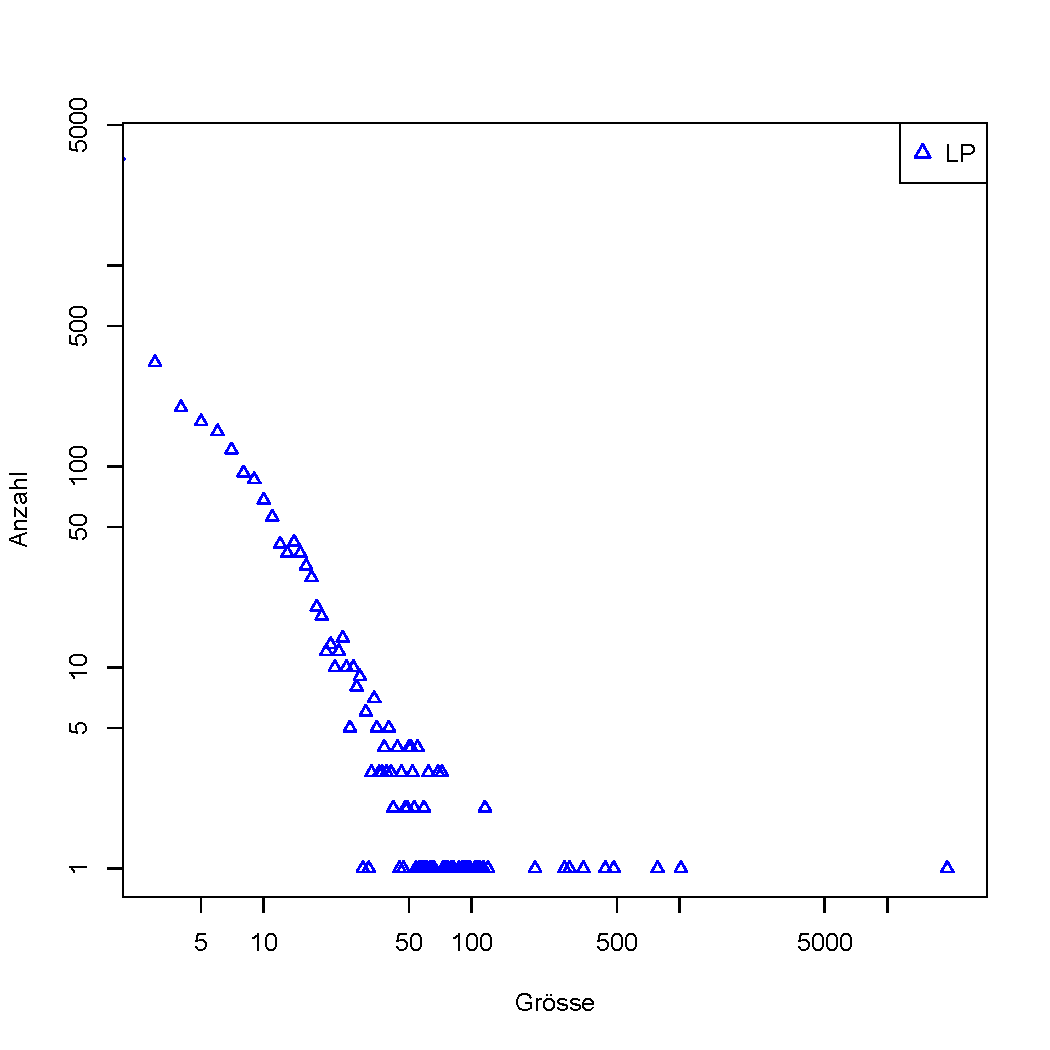
\includegraphics[scale=0.45]{images/community-size-dist_copra1.pdf}}
  \subfloat[]{\label{fig:comsize-copra} 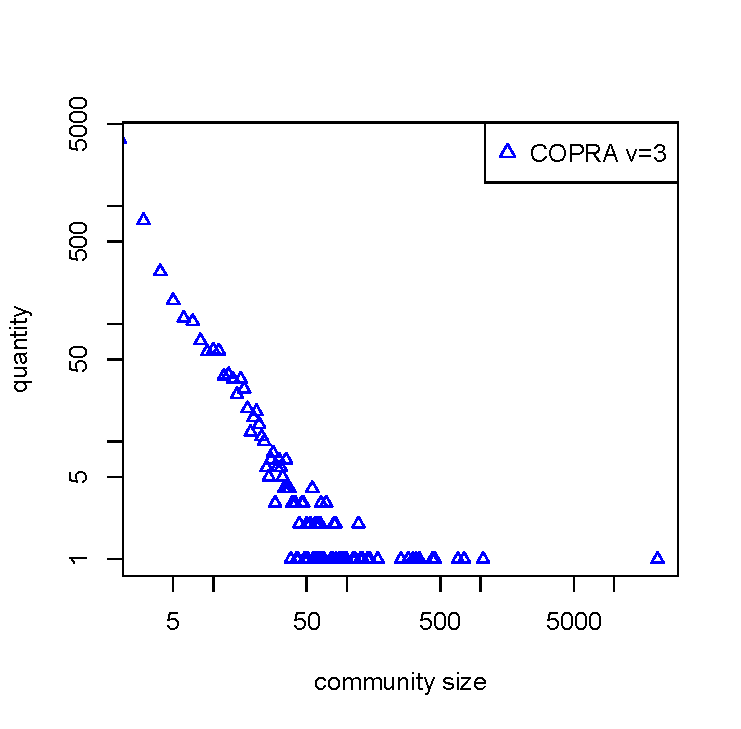
\includegraphics[scale=0.45]{images/community-size-dist_copra.pdf}} \\
  \subfloat[]{\label{fig:comsize-bl2} 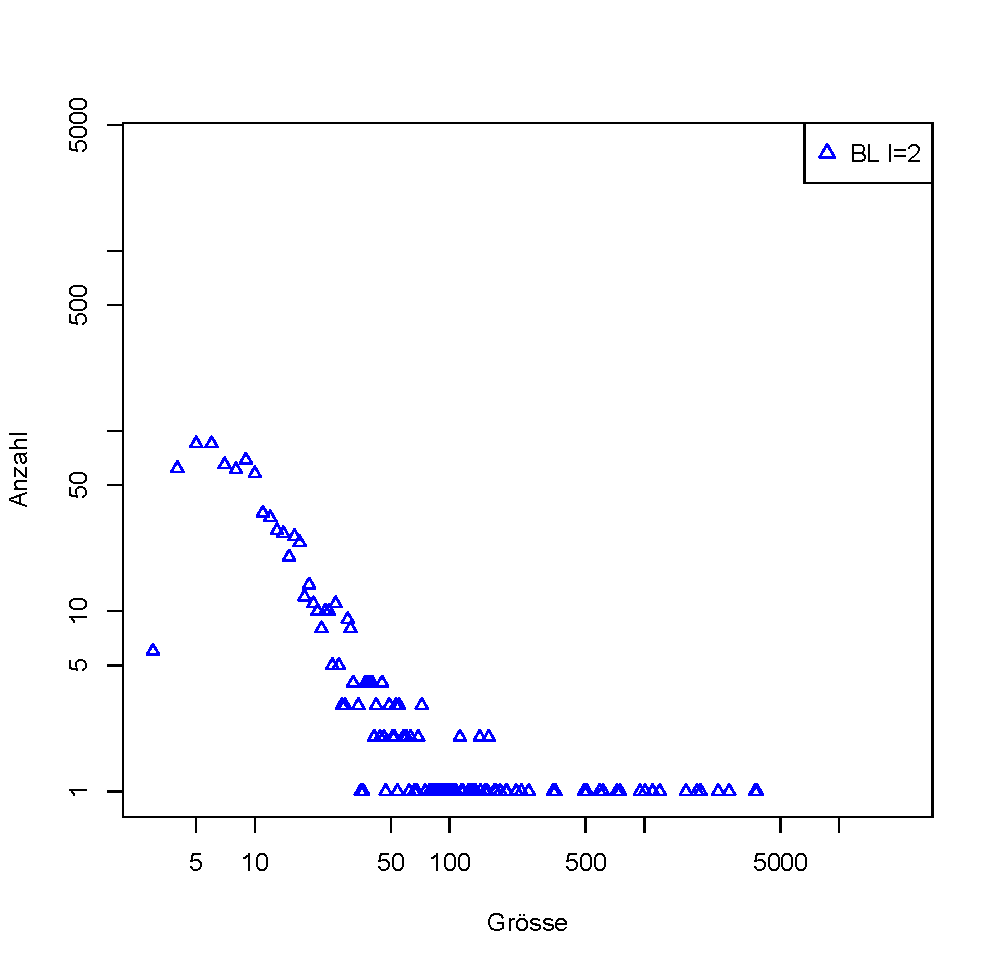
\includegraphics[scale=0.45]{images/community-size-dist_bl2.pdf}} 
  \subfloat[]{\label{fig:comsize-bl5} 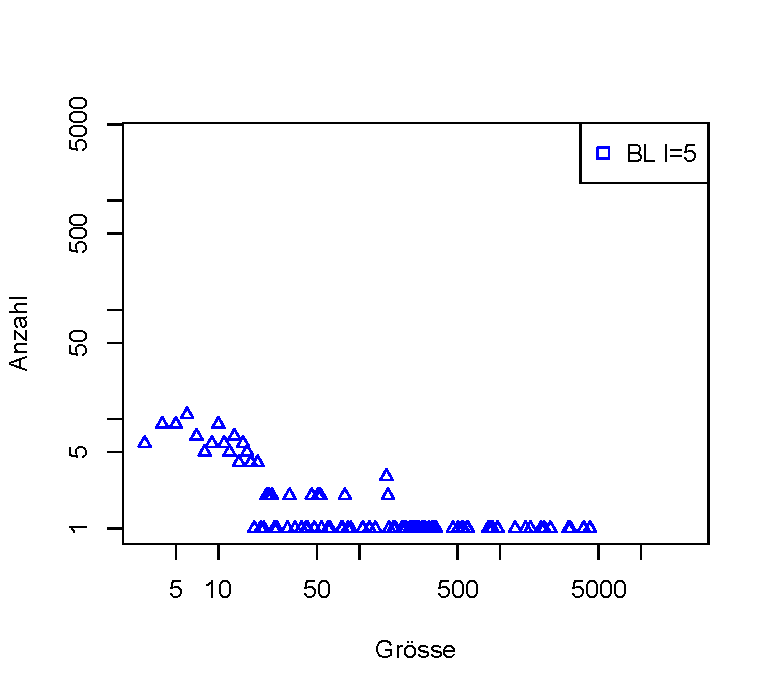
\includegraphics[scale=0.45]{images/community-size-dist_bl5.pdf}} 
  \caption{Verteilung der Größe der Communities}
  \label{fig:comsizedist}
\end{figure}

Wie in Abschnitt
\ref{ch:Grundlagen:sec:Netzwerkanalyse:subsec:Communities}
beschrieben, verläuft der Algorithmus von Blondel et al. iterativ in
Phasen, in denen jeweils zuerst Knoten einer benachbarten Community
zugeordnet werden, wenn sich dadurch ein Modularity-Gewinn erzielen
lässt, und dann die Knoten dieser so entstandenen Communities zu
Knoten in einem neuen Netzwerk verschmolzen werden. Hier werden die
Ergebnisse der Phasen $l=2$ und der letzten Phase $l=5$
betrachtet. Für $l=5$ ergab sich die höchste
Modularity. Allerdings sticht hier die sehr kleine Anzahl von
Communities heraus, die wiederum vergleichsweise groß sein
müssen. Gegenüber dem Ergebnis der Phase 2 ergibt sich eine
relativ kleine Steigerung der Modularity, die mit einem erheblichen
Verlust an \emph{Auflösung} erkauft wird\footnote{Die Zerlegungen
  der Phasen 3 und 4 unterschieden sich nur geringfügig von der
  Zerlegung der Phase 5}. Aus Abbildung \ref{fig:comsize-bl2} und
\ref{fig:comsize-bl5} geht hervor, dass diese Reduktion der Anzahl im
Wesentlichen auf das Reduzieren sehr kleiner Communities
zurückgeht. Da der Algorithmus von Blondel et al. 
mittels einer (lokalen) Optimierung der Modularity arbeitet,
könnte dieses Phänomen auf das in der Literatur beschriebene
Auflösungslimit der Modularity-Funktion (bspw. \cite{Fortunato2007}
\cite{Good2009}) zurückzuführen sein. Es scheint fraglich, ob die
in Relation zur Größe des Graphen sehr geringe Zahl von 186
Communities die Struktur des Graphen (in Bezug auf die inhaltliche
Analyse) adäquat wiedergibt.

\begin{figure}[ht!]
  \centering
  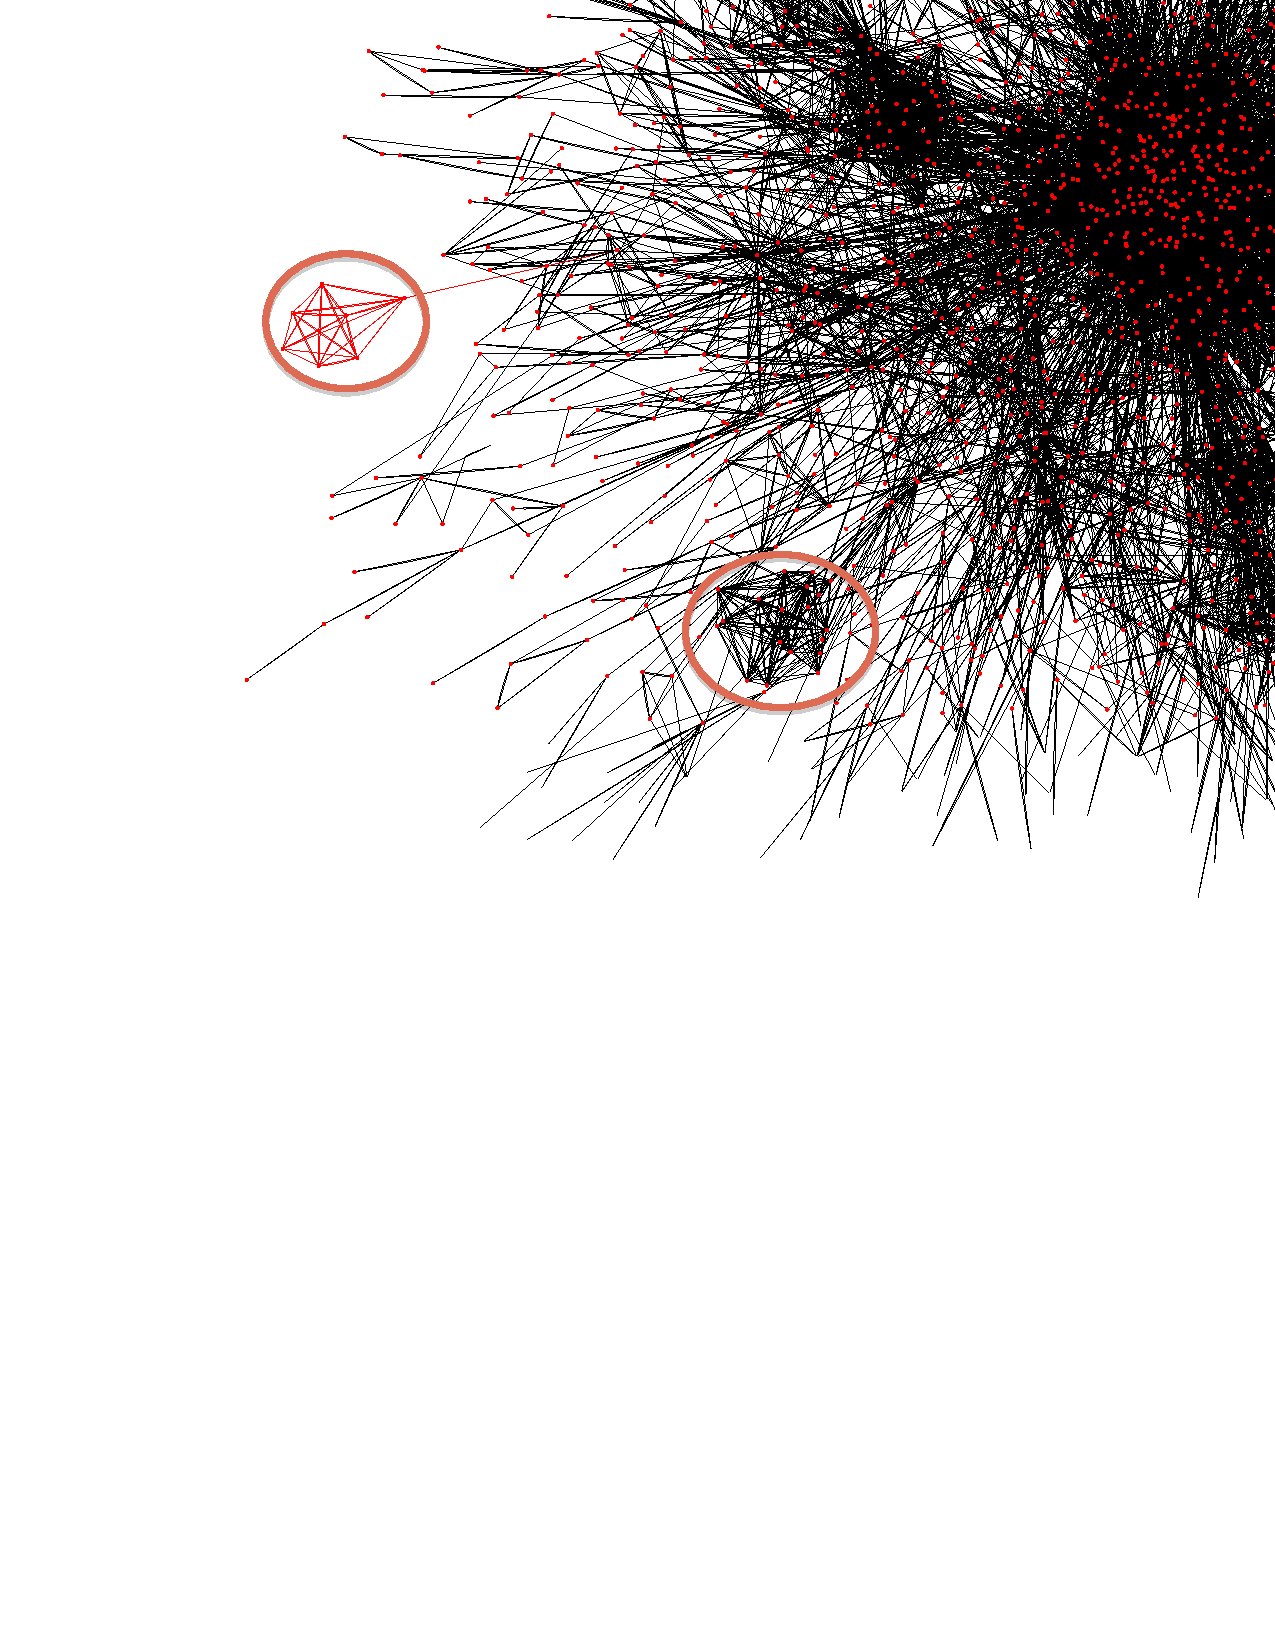
\includegraphics[scale=0.7]{images/blondel-l5-com-c3a5eaab680984b123037897b0be74bf-edit.pdf}
  \caption{Community mit modularen Untereinheiten (Größe 2.271,
    Blondel ($l=5$), Force-directed Layout)}
  \label{fig:large-modular}
\end{figure}

Abbildung \ref{fig:large-modular} illustriert dies anhand einer
Community aus der Zerlegung des Algorithmus von Blondel et al. mit
$l=5$. Diese enthält klar abgegrenzte Untereinheiten, die intuitiv
wieder eigenständige Communities darstellen, sich aber nicht als
solche im Ergebnis wiederfinden.

Die Verteilungen der Community-Größen aus allen Berechnungen sind
in einer Hinsicht konsistent: Neben einer großen Zahl von kleinen
Communities gibt es eine signifikante Anzahl von größeren bis sehr
großen Communities. Es scheint also keine charakteristische Größe
der Communities zu geben.

\begin{table}[t]
  \centering
  \footnotesize
  \begin{tabular}{l|c|c|c}
    Algorithmus & Modularity & Communities &
    Enthaltene Knoten \\
    \hline
    BL ($l=2$)& 0,701 & 936 & 44.934 \\
    BL ($l=5$)& 0,710 & 186 & 44.934 \\
    \hline
    COPRA ($v=1$) & (0,780) & 1.421 & 42.205 \\
    COPRA ($v=3$) & (0,786) & 1.354 & --- \\

  \end{tabular}
  \caption{Modularity-Werte, Anzahl der Communities mit mehr als 3
    Knoten sowie die Anzahl der insgesamt in diesen Communities enthaltenen
    Knoten 
    für die Algorithmen 
    Blondel et al. (BL) in Phase 2 und 5 sowie COPRA mit $v=1$ und
    $v=3$. Die
    Modularity-Werte für COPRA können nicht mit denen für
    Blondel verglichen werden, da ihnen eine andere
    Modularity-Definition für überlappende Communities zugrunde
    liegt.}
  \label{tab:mod-result}
\end{table}

Aus Tabelle \ref{tab:mod-result} geht hervor, dass sich im Fall von
Blondel et al. fast alle Knoten des Graphen in einer Community
wiederfinden, die mindestens die Größe 4 hat. In Abschnitt
\ref{sec:result-allg-merkm-des} wurde gezeigt, dass ein erheblicher
Anteil der Knoten einen sehr geringen Grad von 1 oder 2 hat. Da solche
Knoten mangels Kanten nicht selbst eine dichte Vernetzung herstellen
können, müssen sie Mitglied in Communities sein, in denen Knoten
mit höherem Grad sowohl die interne Vernetzung der Community als
auch die Vernetzung der Community mit anderen erzeugen. COPRA scheint
hingegen dazu tendieren, deutlich mehr Knoten in Communities sehr
kleiner Größe mit 3 oder weniger unterzubringen. Dieses Verhalten
könnte dazu führen, dass die Aussagekraft der Zerlegung in Bezug
auf die realen Communities geschwächt wird, wenn viele Knoten auf
diese Art abgespalten werden.

Gegenüber der COPRA-Zerlegung mit $v=1$ zeigt die Zerlegung mit
$v=3$ eine deutlich grössere Anzahl von Communities der Größe 3
und 4. Abgesehen davon ähneln sich die Verteilungen der Größen aber
weitgehend. Beide enthalten eine charakteristische sehr gro{\ss}e
Community mit ca. 19.000 bzw. ca. 21.000 Mitgliedern. Demgegenüber
bietet die Blondel-Zerlegung mit $l=2$ eine deutlich geringere Anzahl
solcher sehr kleiner Communities, dafür aber eine höhere Zahl
mittlerer (mehr als 100 Mitglieder) und insbesondere eine höhere
Zahl sehr großer (zwischen 500 und 5000 Mitglieder) Communities.  Die
beiden Algorithmen konvergieren nicht gegen ein gemeinsames Optimum,
sondern liefern Ergebnisse, die sich qualitativ stark unterscheiden.

Der insgesamt recht hohe Modularity-Wert weist darauf hin, dass der
Graph in der Tat eine ausgeprägte modulare Struktur hat, wie dies
von einem sozialen Netzwerk erwartet wird. Newman et al. geben an,
dass ein Modularity-Wert $C \ge 0.3$ in der Praxis auf eine
signifikante Community-Struktur schließen lässt \cite{Clauset2004}.

\subsection{Struktur der Communities}
\label{sec:strukt-der-comm}

\begin{figure}[h!]
  \centering
  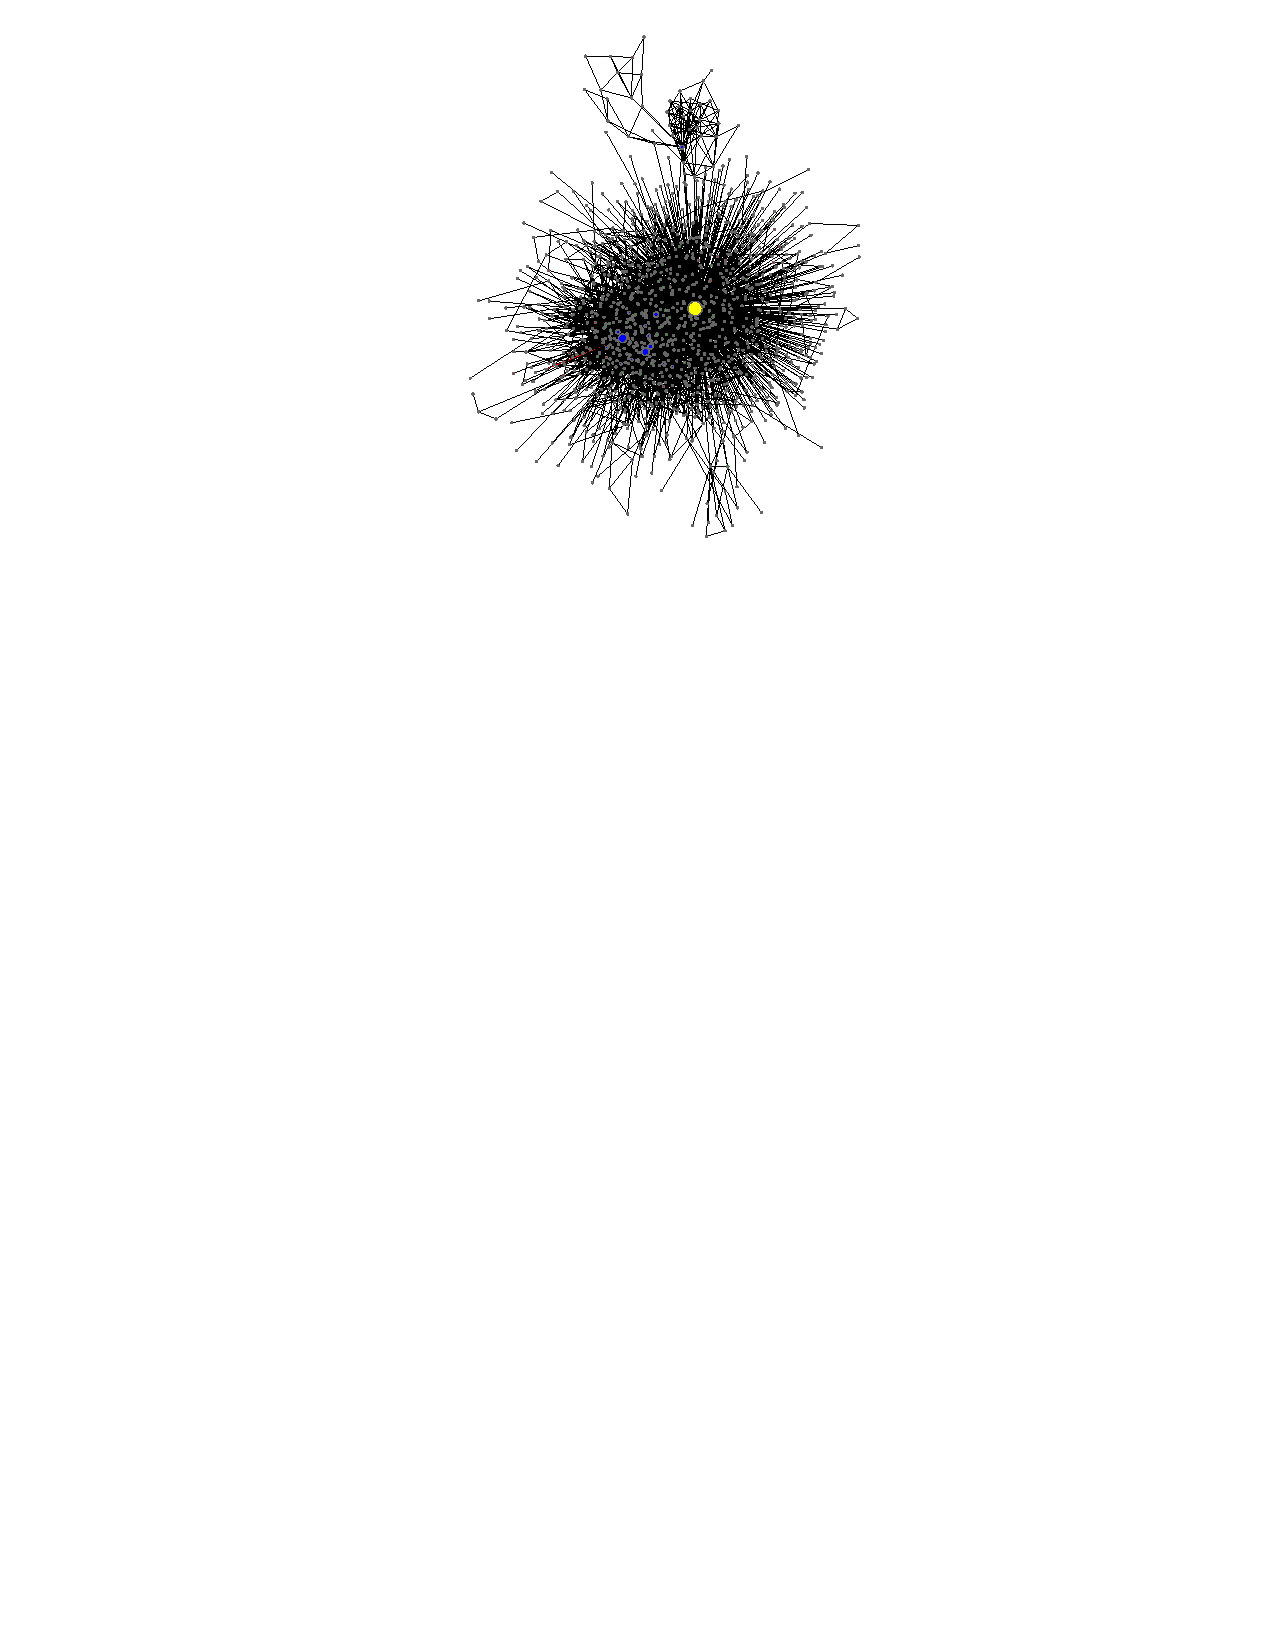
\includegraphics[scale=2]{images/metagraph-copra1-minsize5.pdf}
  \caption{Struktur der Communities (COPRA ($v=1$) (rot: Größe
    $<10$, grün: Größe $<100$, blau: Größe < 1000, gelb:
    Größe > 1000).}
  \label{fig:metagraph-com-copra}
\end{figure}

Die Abbildungen \ref{fig:metagraph-com-copra} und
\ref{fig:metagraph-com-blondel2} zeigen die Struktur der Communities
für die Zerlegungen COPRA ($v=1$) und Blondel ($l=2$). Auffällig
ist hier insbesondere die teilweise sternförmige Struktur der
COPRA-Zerlegung. Ein signifikanter Anteil der kleineren Communities
ist rund um die zentrale Community der Größe ca. 19.000 angeordnet
und im wesentlichen nur mit dieser vernetzt. Diese Struktur weist
gewisse Ähnlichkeiten zur Struktur der starken
Zusammenhangskomponenten auf (siehe Abschnitt
\ref{sec:result-komponentenstruktur}). Diese sind ebenfalls
sternförmig um eine zentrale Komponente angeordnet, die die Größe
der anderen um mehrere Größenordnungen übertrifft. Allerdings
sind im Fall der Community-Struktur noch eine Reihe mittelgroßer
Communities vertreten, die dieses Muster etwas stören. Das
sternförmige Muster der Zusammenhangskomponenten wiederholt sich
also in etwa innerhalb der größten Zusammenhangskomponente auf
einer anderen Ebene. Es könnte daher spekuliert werden, ob das
Netzwerk eine \emph{Selbstähnlichkeit} aufweist, wie sie für eine
Reihe von komplexen Netzwerken gezeigt wurde \cite{Song2005}. Dieser
Frage wurde allerdings im Rahmen dieser Arbeit nicht weiter
nachgegangen. Im Vergleich dazu zeigt sich in der Struktur der
Blondel-Communities die etwas ausgewogenere Verteilung der Größen. Zwar
sind auch hier viele kleine Communities sternförmig um die zentralen
Communities angeordnet, diese verteilen sich hier aber auf mehrere solcher
großen zentralen Communities.

\begin{figure}[h!]
  \centering
  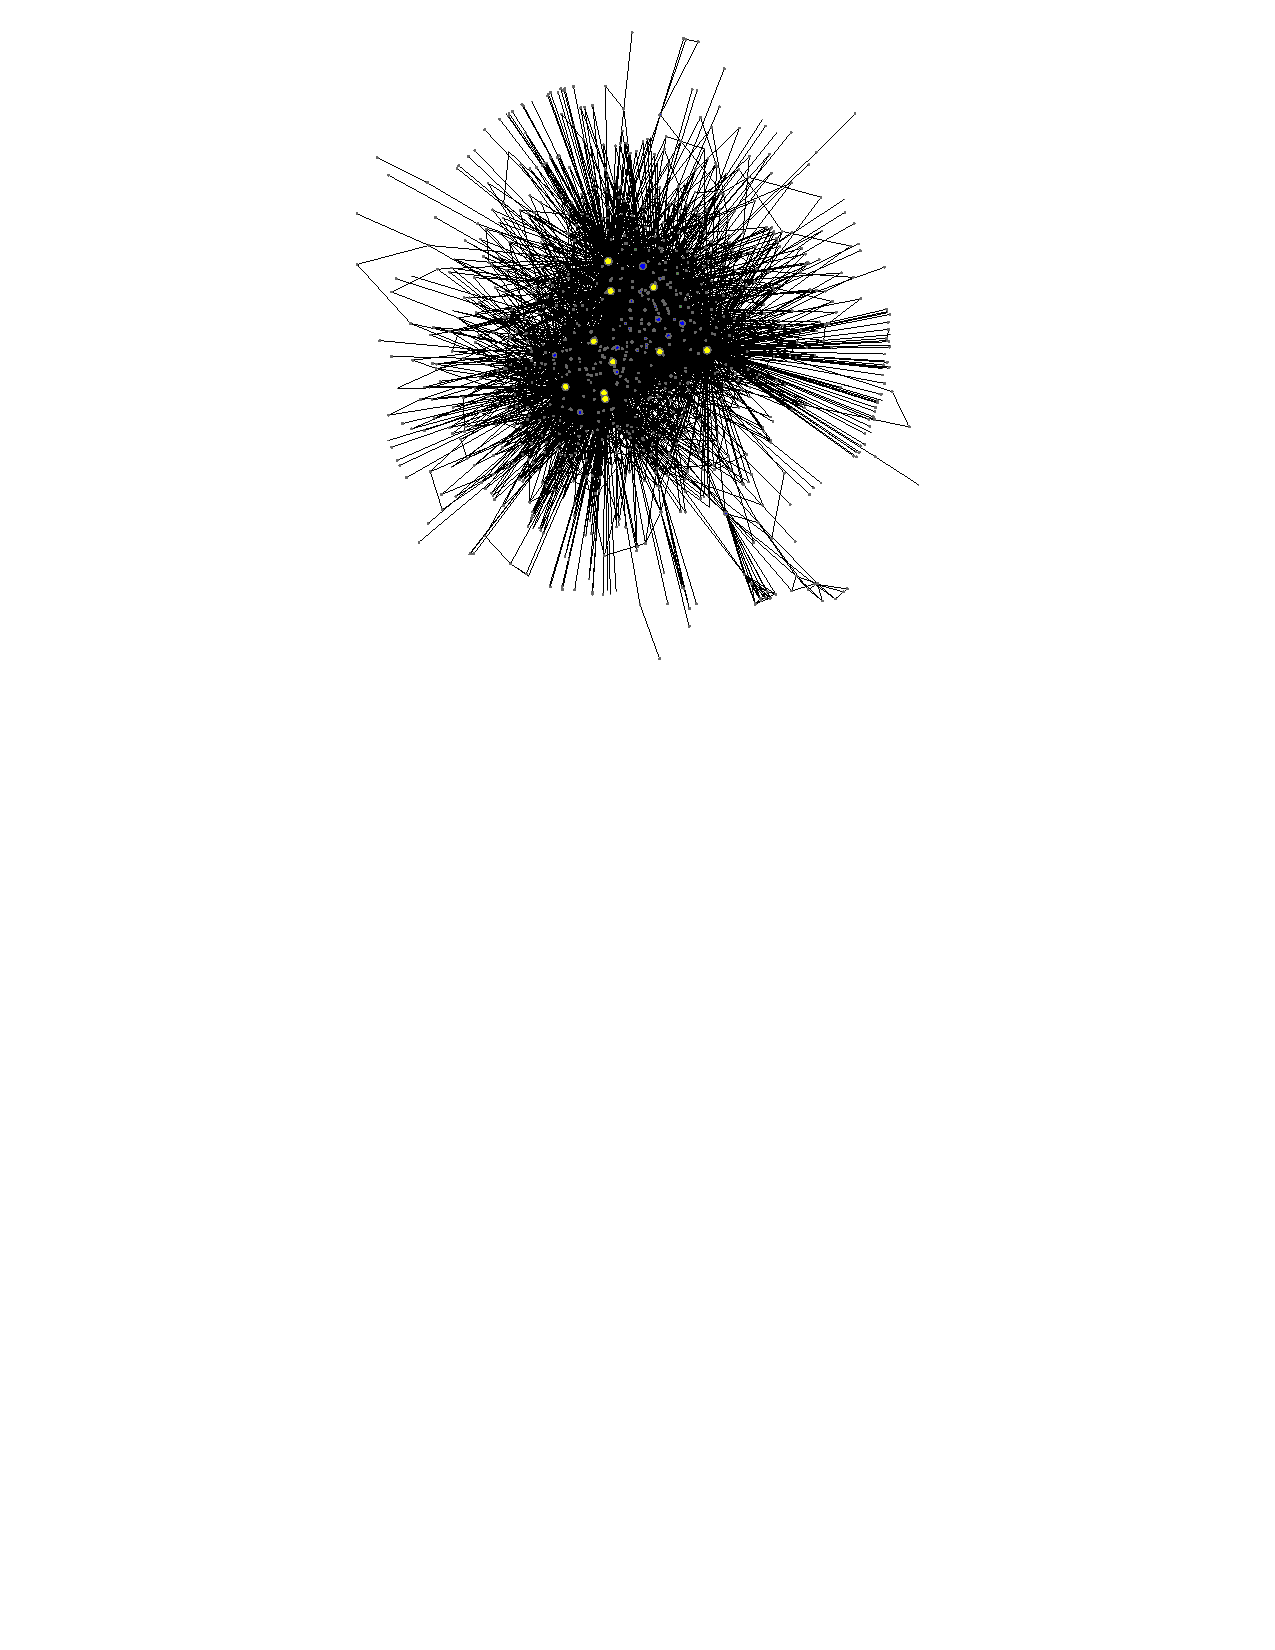
\includegraphics[scale=1.6]{images/metagraph-blondel2-minsize4.pdf}
  \caption{Struktur der Communities (Blondel $l=5$) (Knotenfärbung
    wie in Abb.\ref{fig:metagraph-com-copra})}
  \label{fig:metagraph-com-blondel2}
\end{figure}

\subsection{Inhaltliche Analyse}
\label{sec:inhaltliche-analyse}

\begin{table}[t]
  \centering
  \footnotesize
  \begin{tabular}{l|c|c|c|c|c}
    Algorithmus & TLD-S & TLD-M & SLD-S & SLD-M & SIG \\
    \hline
    BL ($l=2$) & 499 (53\%) & 417 (45\%) & 41 (4\%) & 254 (27\%) & 115 (12\%) \\
    BL ($l=5$) & 85 (47\%) & 85 (47\%) & 15 (8\%) & 38 (21\%) & 26 (14\%) \\
    \hline
    COPRA ($v=1$) & 824 (58\%) & 564 (40\%) & 178 (13\%) & 429 (30\%)
    & 572 (40\%) \\
    COPRA ($v=3$) & 792 (58\%) & 525 (38\%) & 187 (14\%) & 425 (31\%) & 555
    (41\%)
  \end{tabular}
  \caption{Communities, in denen entweder 80\% (TLD-S) oder 40\%
    (TLD-M) der UserIDs in der gleichen TLD bzw. in der gleichen SLD
    (SLD-S/SLD-M) liegen oder in denen mindestens 80\% der Signaturen
    innerhalb eines Monats entstanden sind (SIG).}
  \label{tab:assign}
\end{table}

Aus Tabelle \ref{tab:assign} geht hervor, dass für alle Zerlegungen
fast alle Communities einer Top-Level-Domain zuordenbar sind oder von
einer TLD dominiert werden. Werden die generischen Top-Level-Domains
(gTLD: com, org, net, info, ...) abgezogen, verbleiben im Fall von COPRA
noch 519 (38\%) Communities, die einer TLD (und damit einer
\emph{Country-Coded TLD (ccTLD)}) zugeordnet werden können und 315
(23\%), die von einer ccTLD dominiert werden. Für die anderen
Zerlegungen ergeben sich ähnliche Werte. Damit ist immerhin etwa die
Hälfte der Communities einem Land zuordenbar. Für die von einer
gTLD dominierten Communities ergeben Stichproben, dass sich die
Teilnehmer der meisten dieser Communities anhand der Namen zumindest
einem Sprachraum zuweisen lassen.

Dieses Ergebnis ist naheliegend. Wie in Abschnitt
\ref{sec:community-analyse} dargelegt, wird davon ausgegangen, dass
ein wesentlicher Faktor, der das Zustandekommen von Signaturen
beeinflusst, die sozialen Kontakte einer Person sind. Es ist weiterhin
naheliegend, dass sich diese sozialen Kontakte unter anderem aufgrund
von Sprachbarrieren und der räumlichen Nähe hauptsächlich im
Rahmen eines Landes ergeben. Beispielsweise ist für eine aus
Finnland stammende Person anzunehmen, dass die Mehrzahl ihrer Freunde,
Bekannten, Geschäftspartner und sonstigen Kontakte wieder Finnen
sind.

Zwar könnte argumentiert werden, dass das Internet die geographische
bzw. nationale Beschränkung sozialer Kontakte aufhebt. Allerdings
spielt die geographische Nähe eine wichtige Rolle im
Signaturprozess. Die verbreitete Prozedur für das Signieren eines
Schlüssels setzt ein direktes persönliches Treffen der
Signierenden voraus (siehe Abschnitt \ref{sec:sozi-komp-des}). Es ist
anzunehmen, dass die überwiegende Mehrheit der PGP-Benutzer die
meiste Zeit in einem Land und damit in einem geographisch
eingegrenzten Bereich verbleibt. Damit kommen für diese Mehrheit
überwiegend nur Bewohner des gleichen Landes als Signaturpartner in
Frage. Als Mechanismen für die internationale Vernetzung kommen dann
etwa internationale Konferenzen in Frage. Nur ein sehr kleiner Teil
der PGP-Benutzer dürfte die notwendige internationale Mobilität
aufweisen, so dass sich seine Signaturen nicht überwiegend einem
geographischen Bereich bzw. einem Land zuweisen lassen.

Interessanter für die Fragestellung ist aber die Erkennung von
Keysigning-Parties und die Zuordnung zu Second-Level-Domains. Im
Vergleich der Algorithmen (Tabelle \ref{tab:assign}) zeigt sich
zunächst, dass die COPRA-Zerlegungen bessere Resultate liefern als
die Blondel-Zerlegungen, da hier mehr Communities zugeordnet werden
können. Zwar entfällt bei COPRA ein großer Anteil dieser
Zuordnungen auf sehr kleine Communities der Größe 3 und 4. Die
Aussagekraft solcher kleiner Zuordnungen ist selbstverständlich sehr
begrenzt. Werden diese abgezogen, verbleibt aber immer noch eine
grössere Zahl zuordnenbarer Communities von signifikanter Größe. 

Aus den absoluten Zahlen in Tabelle \ref{tab:assign} und den
Verteilungen der Größen in Abbildungen \ref{fig:sld-suredist},
\ref{fig:sld-maybedist} und \ref{fig:time-corrdist} geht hervor, dass
die \"uberlappende Zerlegung keine wesentlichen Vorteile bringt, da
nicht eine deutlich gr\"ossere Anzahl von Communities inhaltlich
zugeordnet werden kann. 

Im Vergleich der Blondel-Zerlegungen zeigt sich, dass das
Zusammenpacken von Communities von Phase $l=2$ zu Phase $l=5$ und der
damit verbundene Auflösungsverlust es erheblich erschwert, die
Communities inhaltlich zuzuordnen. Eine Zerlegung mit höherer
Modularity entspricht also nicht im Allgemeinen einer Zerlegung, die
die Struktur realer Communities besser wiedergibt. Die Zerlegungen des
Algorithmus von Blondel et al. scheinen insgesamt vom
Auflösungslimit der Modularity-Maximierung betroffen zu sein und
bieten daher nicht die notwendige Auflösung, um die Communities
besser inhaltlich analysieren zu können.

Insgesamt ist eine tatsächliche Zuordnung anhand des
80\%-Schwellwerts nur für sehr wenige Communities von geringer
Größe möglich. Für den 40\%-Schwellwert und die zeitliche
Korrelation ist die Anzahl zuordnenbarer Communities deutlich
höher. Auch hier entfällt allerdings die Mehrzahl auf sehr kleine
Communities.  Dass so gut wie keine Communities mit einer Größe
über 100 zugeordnet werden können, spricht dafür, dass diese
sich nicht anhand dieser einfachen Mechanismen bilden.

Die sehr große Community aus der COPRA-Zerlegung könnte vermuten
lassen, dass hier relativ willkürlich Knoten zusammengepackt
wurden. Allerdings hat diese Community eine Reihe von Eigenschaften,
die nahe legen, dass diese Gruppierung durchaus Sinn ergibt. Von 21.157
Knoten verfügen 8.879 (42\%) über eine E-Mail-Adresse in der
Top-Level-Domain \emph{.de}, während andere -- insbesondere
nicht-deutschsprachige -- ccTLDs deutlich schwächer vertreten
sind. Das zeigt einerseits einen überraschend hohen Anteil von
deutschen oder deutschsprachigen Benutzern am Gesamtnetzwerk. Die 8.879
Schlüssel sind natürlich nur eine Untergrenze, da auch in einer
Vielzahl weiterer Communities deutsche Teilnehmer vorkommen. Ein Grund
für diese hohe Anzahl deutscher Schlüssel könnte in der in
Abschnitt \ref{sec:sozi-komp-des} erwähnten "`Krypto-Kampagne"' der
Zeitschrift c't liegen, die das Bewusstsein für die Notwendigkeit
der Authentifizierung von Schlüsseln im deutschsprachigen Raum
deutlich gesteigert haben dürfte. Andererseits lässt dies den
Schluss zu, dass die enthaltenen Knoten eben nicht willkürlich
zusammengepackt wurden, sondern neben ihrer topographischen Nähe
auch eine "`inhaltliche"' Gemeinsamkeit aufweisen. Darauf weist auch
hin, dass in dieser Community eine relativ zu anderen SLDs sehr große
Anzahl von Schlüsseln von Mitgliedern des Debian-Projekts enthalten
ist. Diese Community enthält nicht nur knapp die Hälfte der
Schlüssel, sondern mit ca. 260.000 Kanten den Großteil der
überhaupt vorhandenen Kanten. Sie ist also anscheinend intern sehr
dicht vernetzt. Es scheint daher fraglich, ob sich innerhalb dieser
Community wieder eine ausgeprägte Community-Struktur finden lässt.

\begin{table}
  \centering
  \begin{tabular}{c|c|c}
    Größe & SLD & Anteil \\
    \hline
    436 & apache.org & 48\% \\
    130 & nun.org & 82\% \\
    97 & cert.org & 70\% \\
    81 & redhat.org & 68\% \\
    63 & purdue.edu & 65\% \\
    59 & cisco.com & 79\% 
  \end{tabular}
  \caption{Die größten, von einer SLD dominierten Communities
    (COPRA).}
  \label{tab:ass-examples}
\end{table}
In Tabelle \ref{tab:ass-examples} sind die 6 größten Communities
aus der COPRA-Zerlegung mit Zuordnung zu Second-Level-Domains
aufgeführt. Diese stammen sämtlich aus einem technologischen oder
akademischen Umfeld.

\subsection{Kriterium für KSPs}
\label{sec:kriterium-fur-ksps}

\begin{figure}[th!]
  \centering
  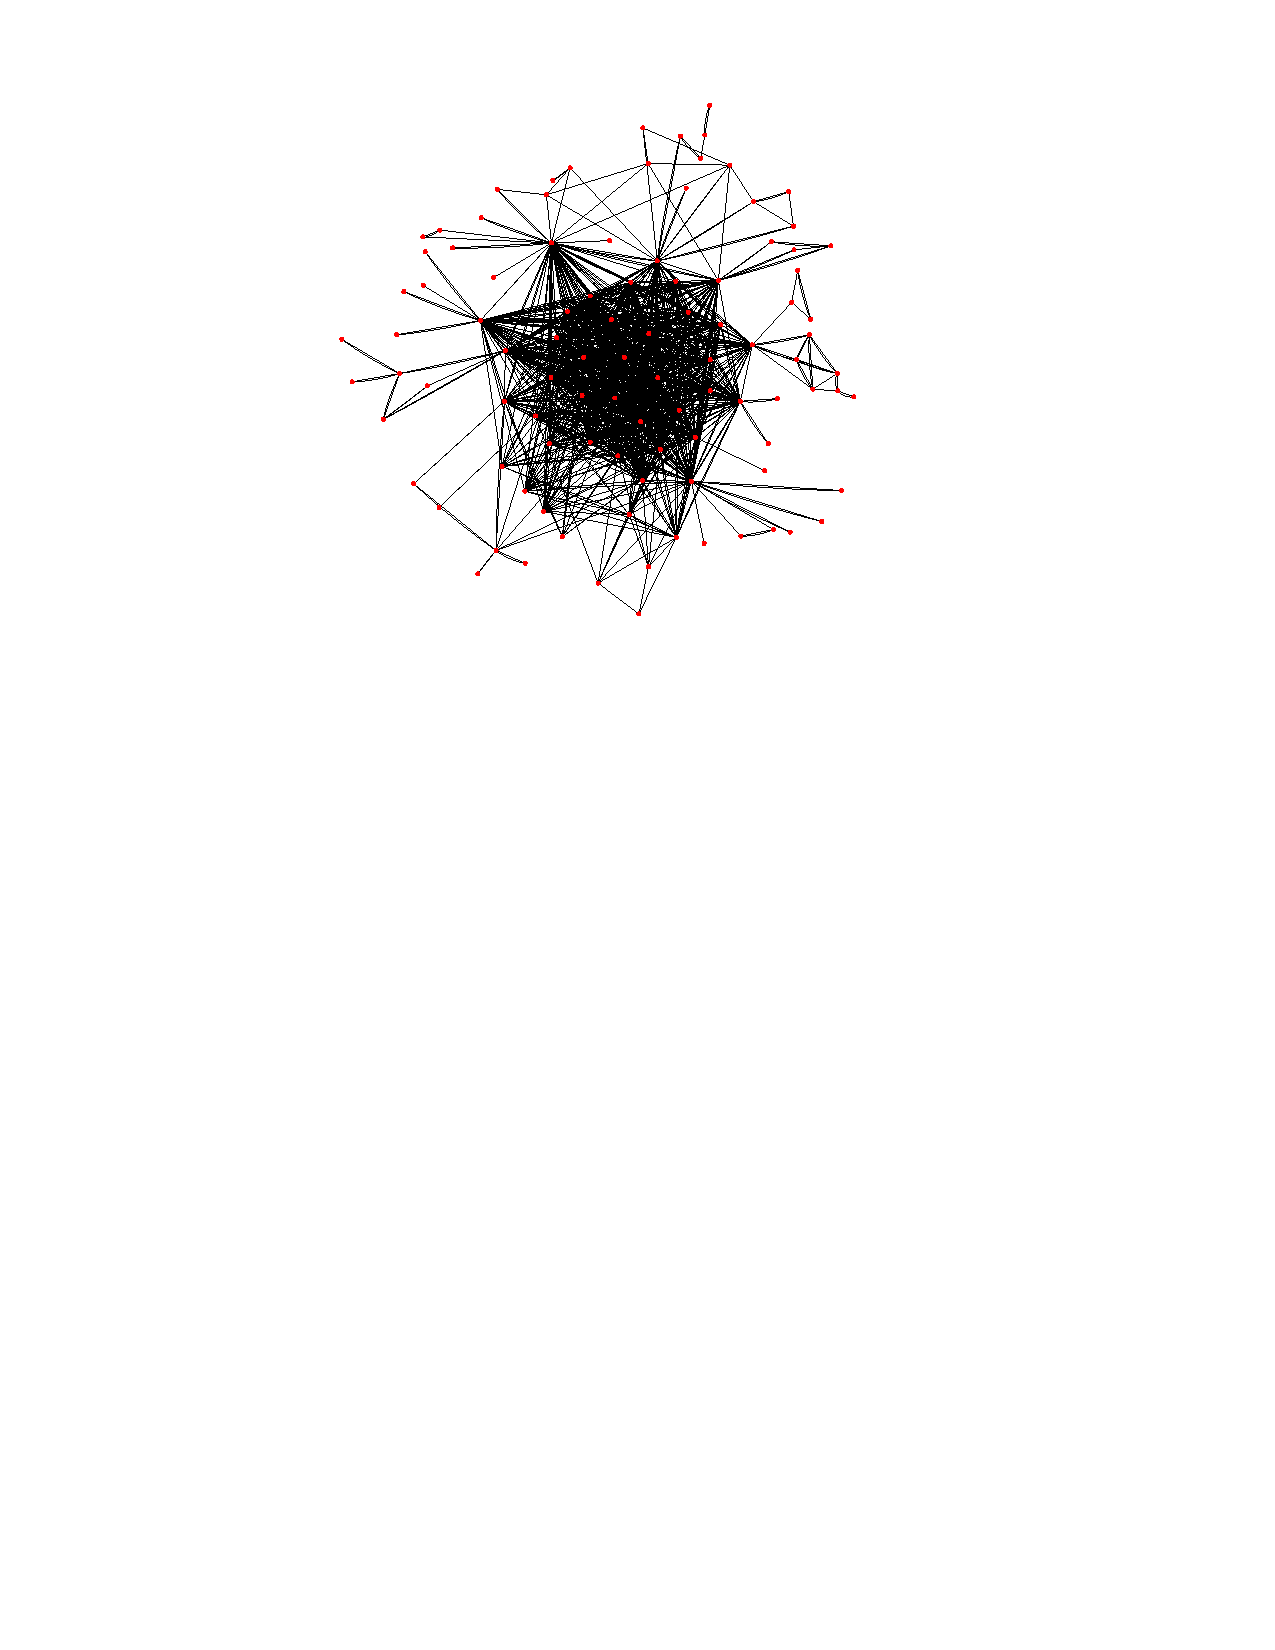
\includegraphics[scale=1.5]{images/subgraph-label-time-fa62cc57cd35e9f90b85435efc407ad5.pdf}
  \caption{Community mit zeitlicher Korrelation der Signaturen
    (Blondel $l=5$),
    100 Knoten, 72\% der Signaturen innerhalb eines Monats)}
  \label{fig:time-corr-com-normal}
\end{figure}

\begin{figure}[th!]
  \centering
  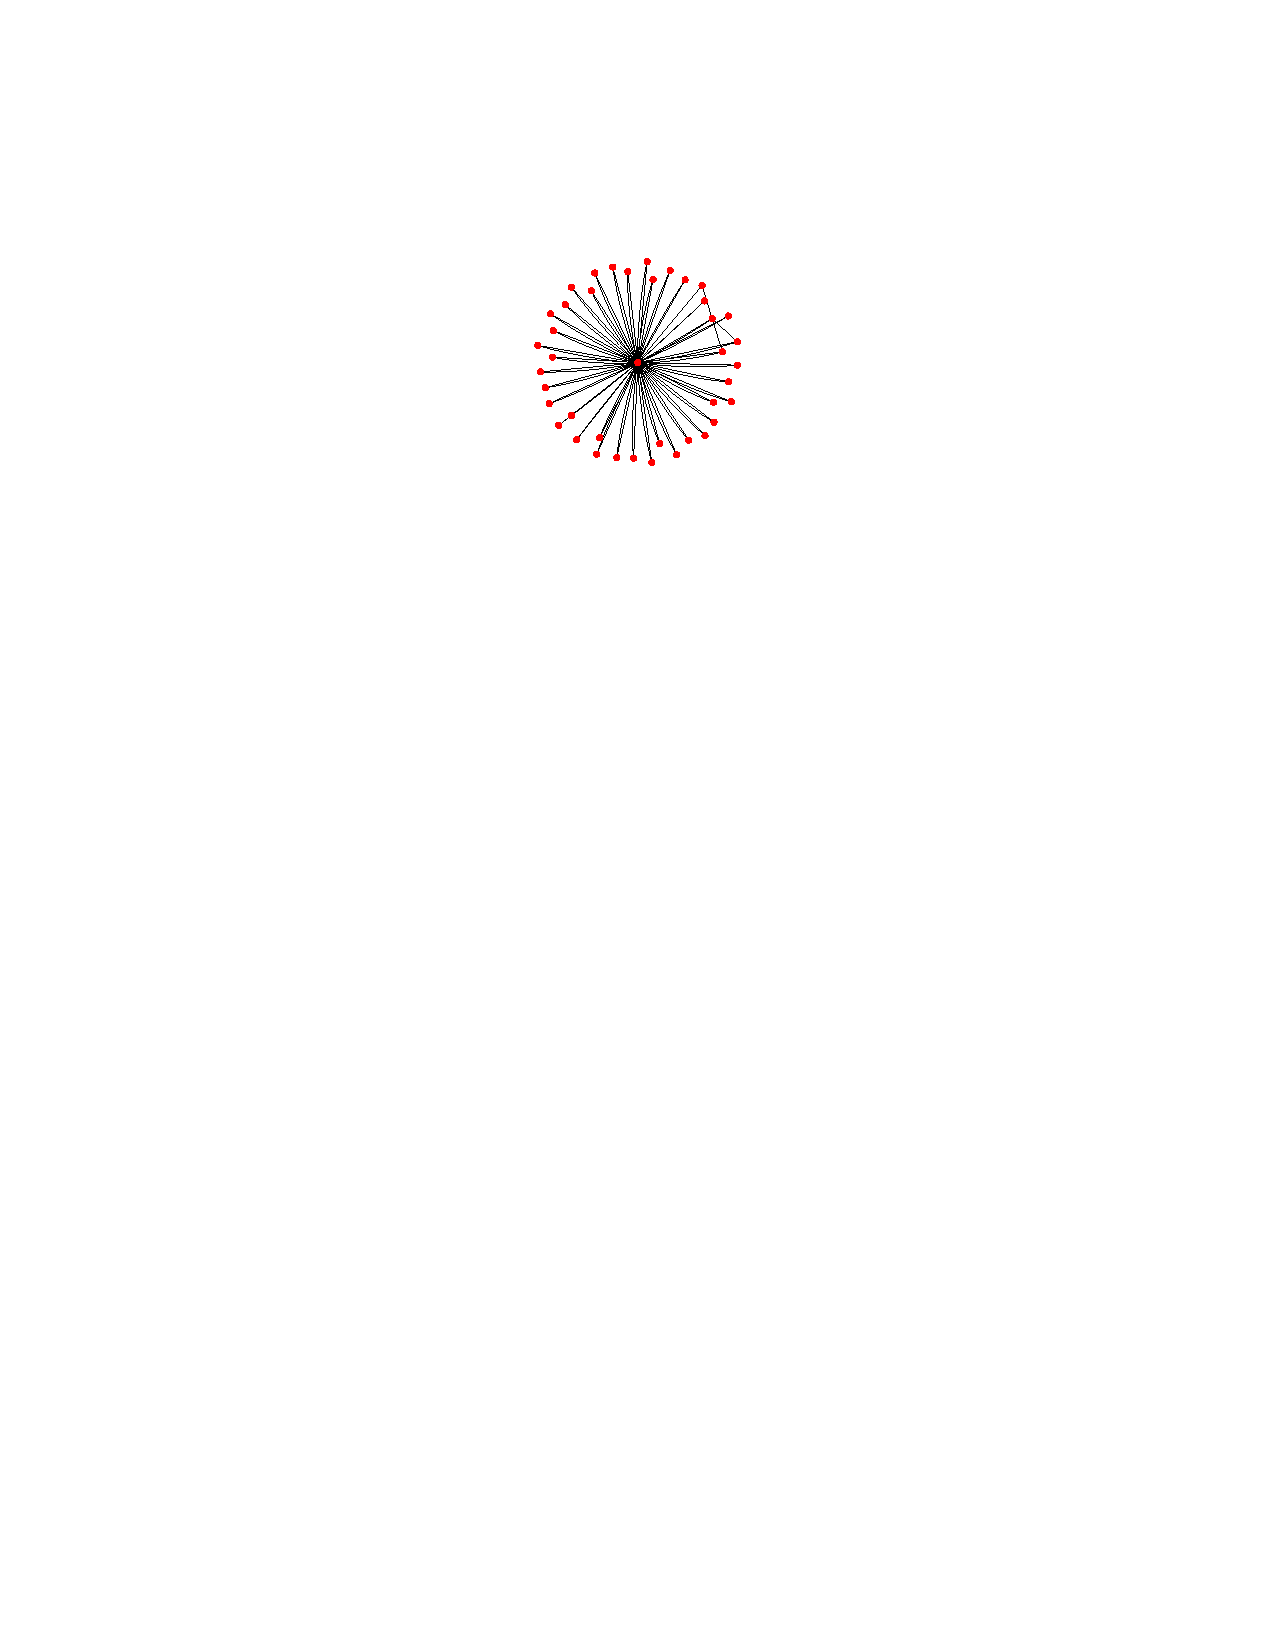
\includegraphics[scale=1.3]{images/label-subgraph-41-star-c222345bc5eb1f9eff80d58a81861974.pdf}
    \caption{Community mit zeitlicher Korrelation der Signaturen
      (Blondel ($l=5$),
      41 Knoten, 84 \% der Signaturen innerhalb eines Monats)}
  \label{fig:time-corr-com-star}
\end{figure}

Es stellt sich die Frage, ob die zeitliche Korrelation der Signaturen
in einer Community ein geeignetes Mittel ist, um Keysigning-Parties zu
erkennen. Neben dem zeitlichen Zusammenhang der Signaturen ist ein
weiteres Merkmal einer Keysigning-Party wie in
Ab. \ref{sec:sozi-komp-des} beschrieben, dass jeder Teilnehmer mit
(fast) jedem anderem Teilnehmer Signaturen austauscht, so dass sich
eine fast vollständige Vermaschung -- fast eine Clique --
ergibt. Eine stichprobenartige Untersuchung in den Communities zeigt,
dass die meisten Communities mit zeitlicher Korrelation zumindest
teilweise dieses Merkmal zeigen. Abbildung
\ref{fig:time-corr-com-normal} zeigt ein Beispiel einer solchen
Community. Etwa die Hälfte der Knoten ist in einer Fast-Clique
enthalten, deren Knoten mit (fast) allen anderen vernetzt sind. Dieser
innere Teil des Teilgraphen entspricht genau dem Bild, das als
Resultat einer Keysigning-Party erwartet wird. Auch wenn dies auf die
meisten der Communities mit zeitlicher Korrelation zutrifft, gibt es
auch Gegenbeispiele. Abbildung \ref{fig:time-corr-com-star} zeigt eine
Community, die zwar das Kriterium der zeitlichen Korrelation
erfüllt, ansonsten aber nichts mit dem erwarteten Bild einer
Keysigning-Party gemein hat. Allerdings erfüllt der Teilgraph
trotzdem das Kriterium der Community, da die Knoten am Rand nur
Signaturen zu dem zentralen Knoten haben und damit die interne
Kantendichte deutlich höher ist als die externe. Um solche
Extremfälle auszuschließen, ist als zusätzliches Kriterium für
die Erkennung von Keysigning-Parties ein hoher durchschnittlicher Grad
der Knoten denkbar.

\begin{figure}[th!]
  \centering
  \subfloat[]{\label{fig:sld-sure-copra1} 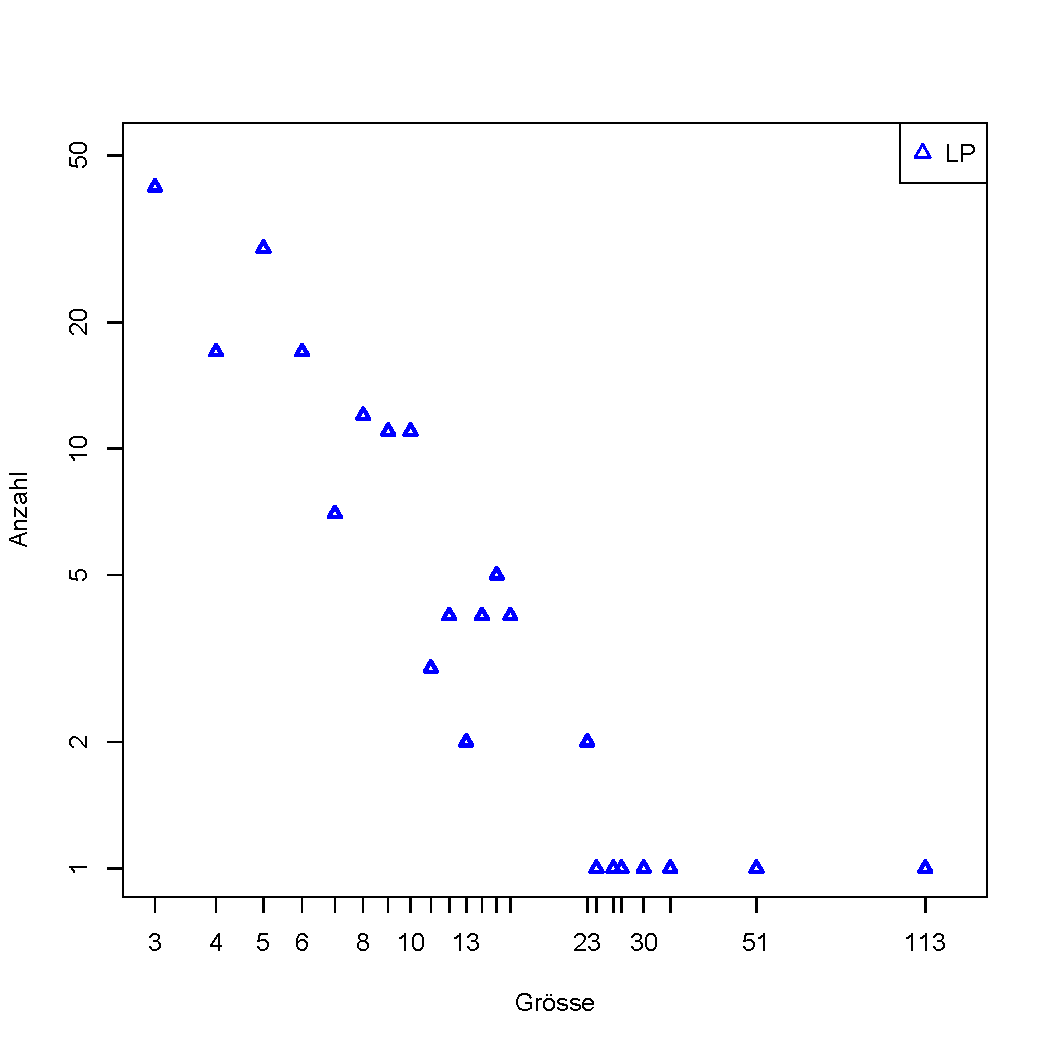
\includegraphics[scale=0.45]{images/sld-sure-ass_copra1.pdf}}
  \subfloat[]{\label{fig:sld-sure-bl2} 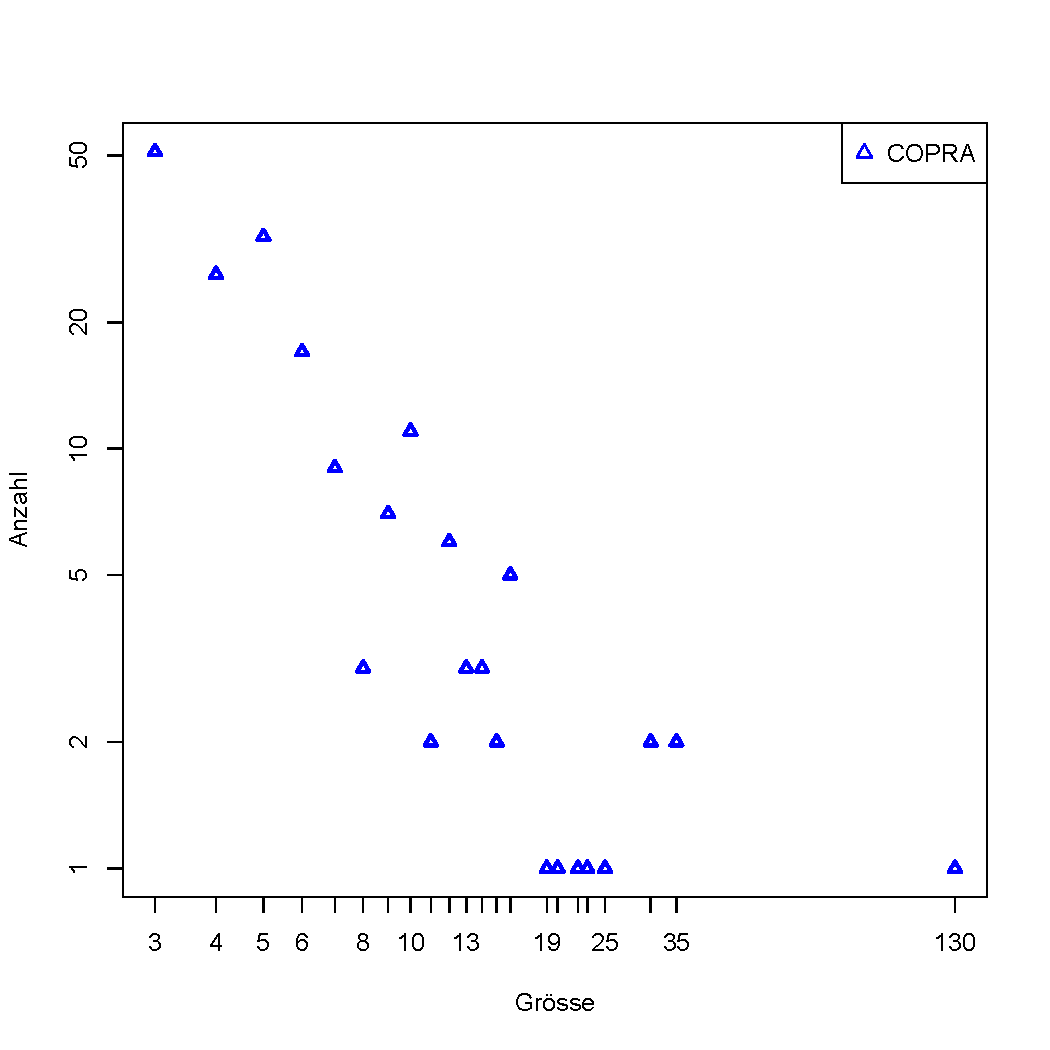
\includegraphics[scale=0.45]{images/sld-sure-ass_copra.pdf}}\\
  \subfloat[]{\label{fig:sld-sure-bl5} 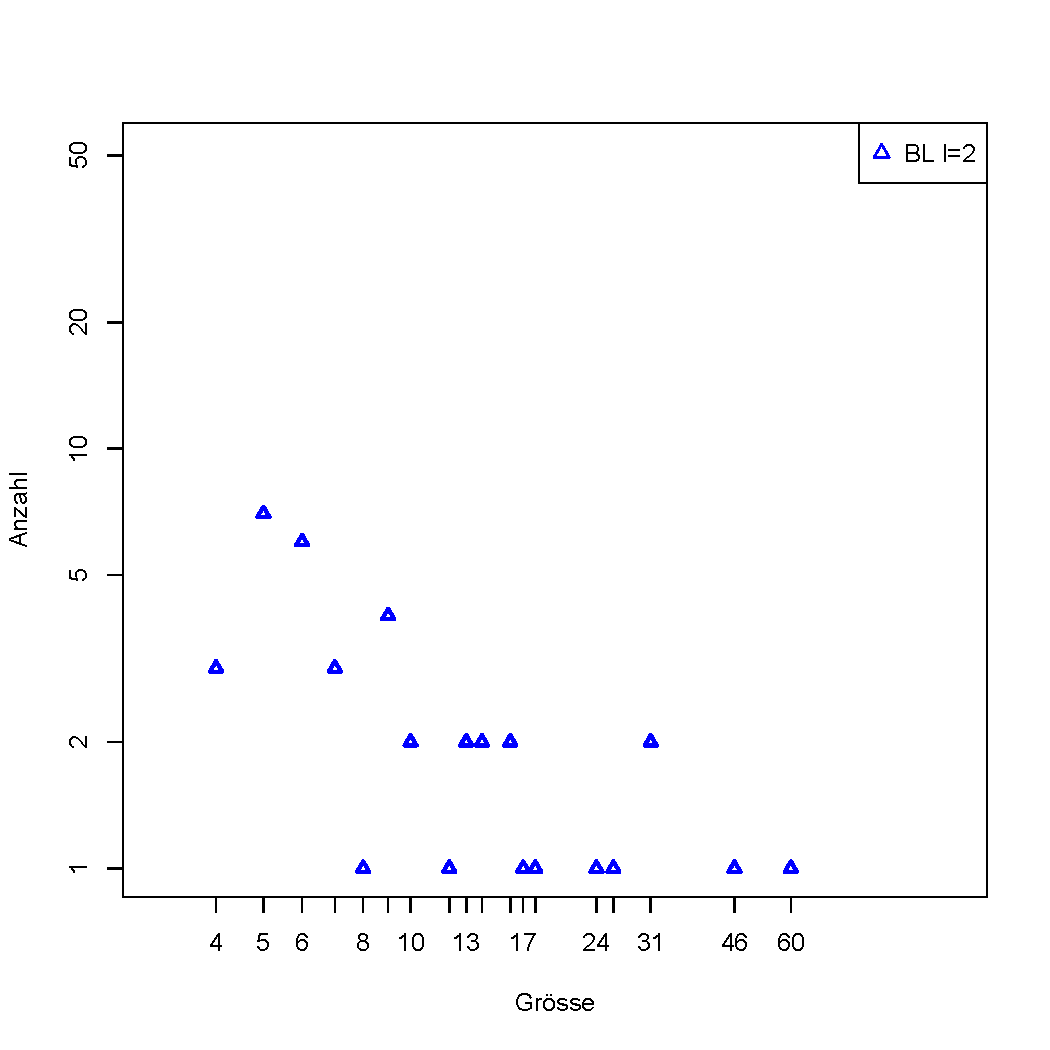
\includegraphics[scale=0.45]{images/sld-sure-ass_bl2.pdf}} 
  \subfloat[]{\label{fig:sld-sure-copra} 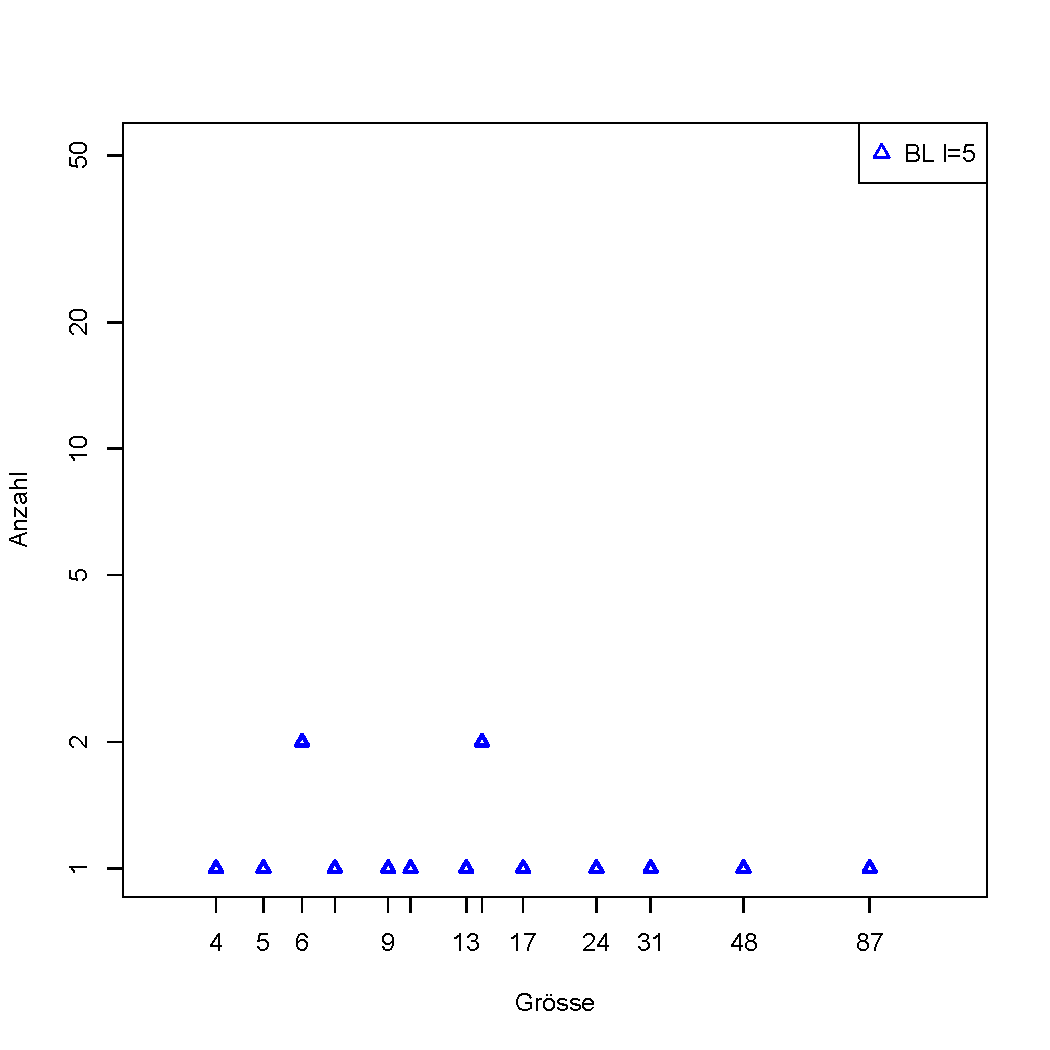
\includegraphics[scale=0.45]{images/sld-sure-ass_bl5.pdf}}
  \caption{Zuweisung von Domains zu SLDs abhängig von der
    Community-Größe.}
  \label{fig:sld-suredist}
\end{figure}

\begin{figure}[th!]
  \centering
  \subfloat[]{\label{fig:sld-maybe-copra1} 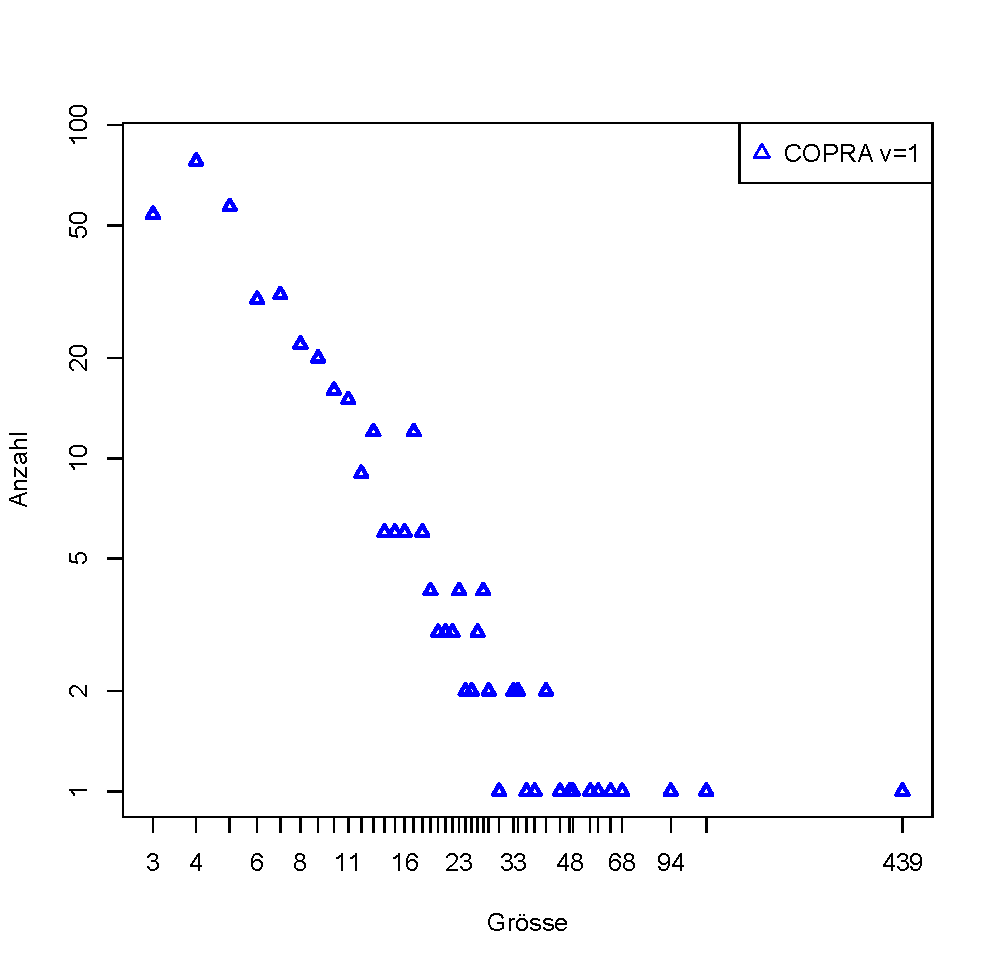
\includegraphics[scale=0.45]{images/sld-maybe-ass_copra1.pdf}}
  \subfloat[]{\label{fig:sld-maybe-bl2} 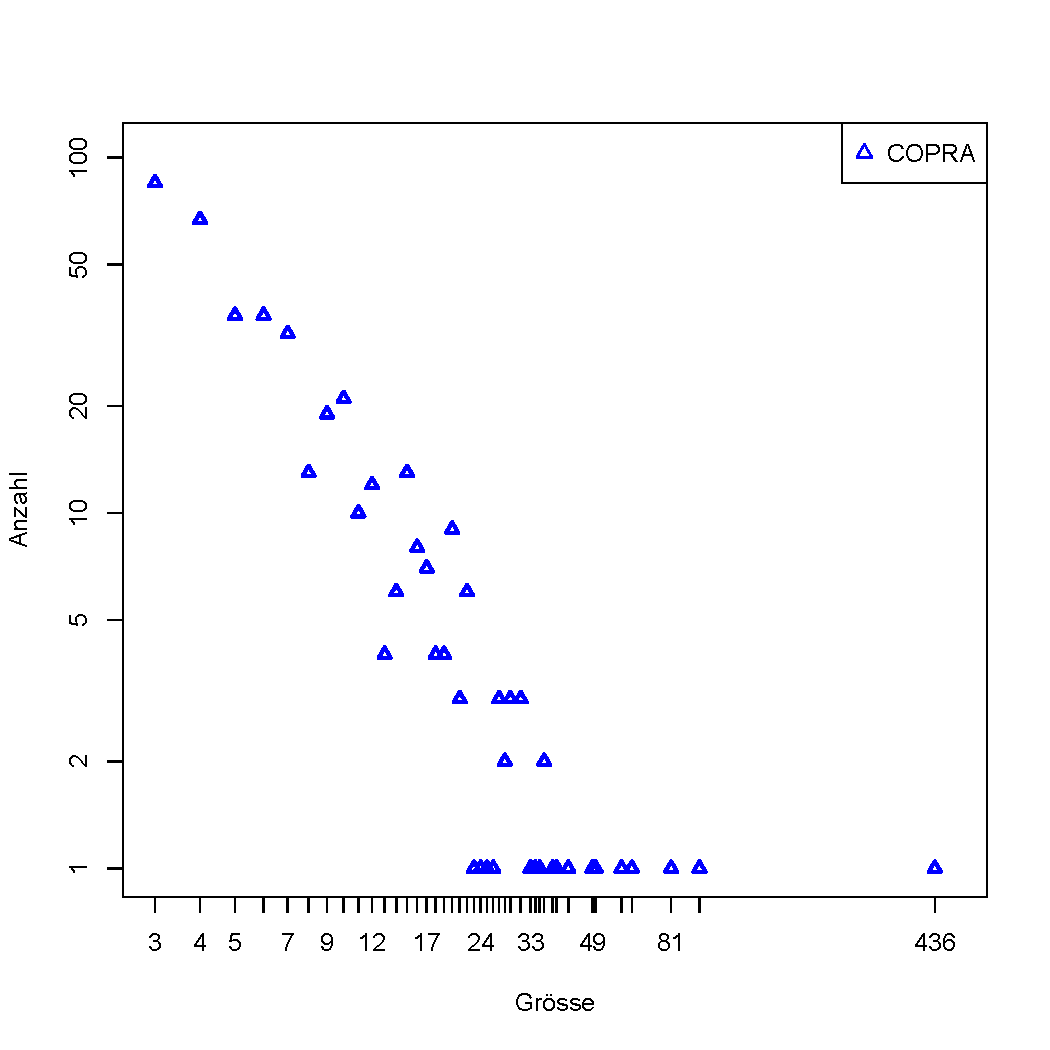
\includegraphics[scale=0.45]{images/sld-maybe-ass_copra.pdf}}\\
  \subfloat[]{\label{fig:sld-maybe-bl5} 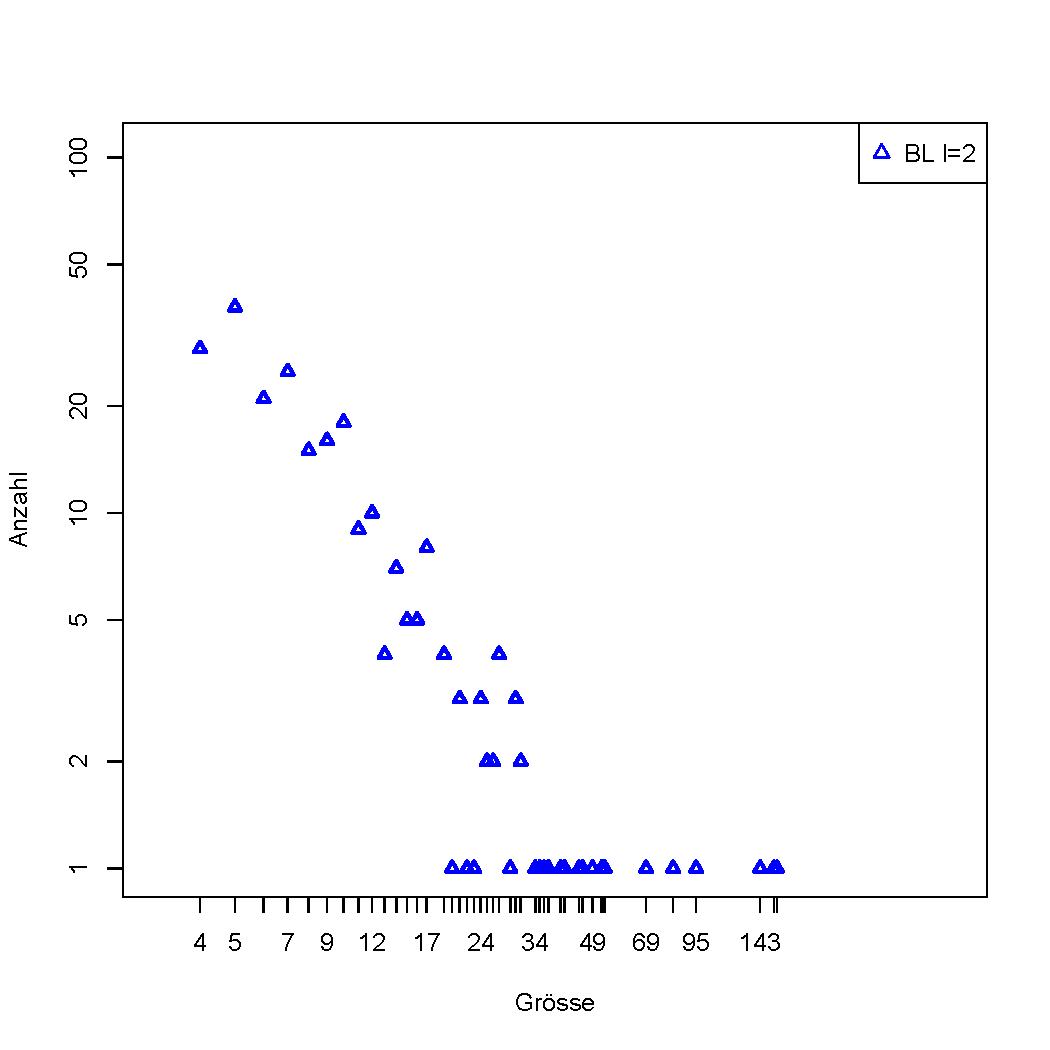
\includegraphics[scale=0.45]{images/sld-maybe-ass_bl2.pdf}} 
  \subfloat[]{\label{fig:sld-maybe-copra} 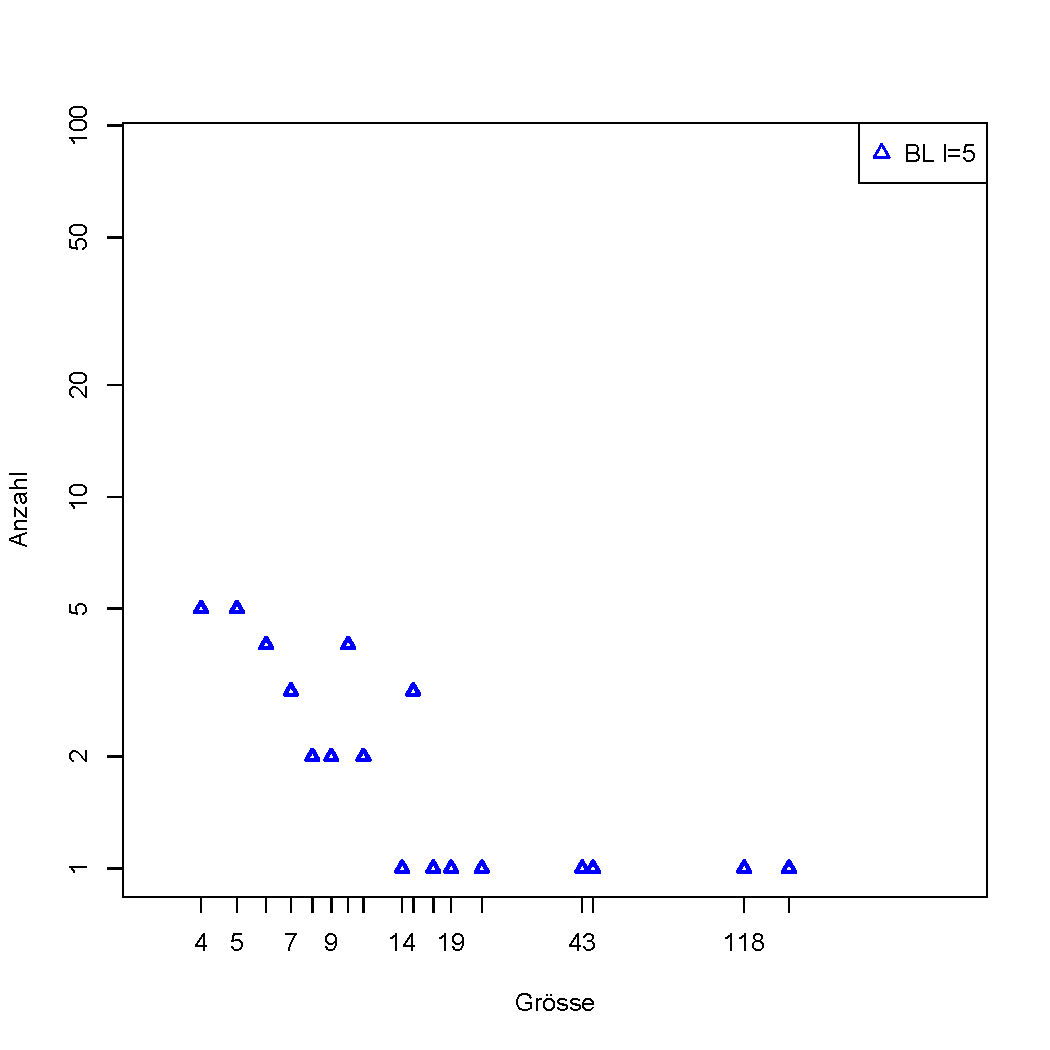
\includegraphics[scale=0.45]{images/sld-maybe-ass_bl5.pdf}}
  \caption{Verteilung der Größe der von einer SLD dominierten
    Communities.}
  \label{fig:sld-maybedist}
\end{figure}

\begin{figure}[th!]
  \centering
  \subfloat[]{\label{fig:time-corr-copra1} 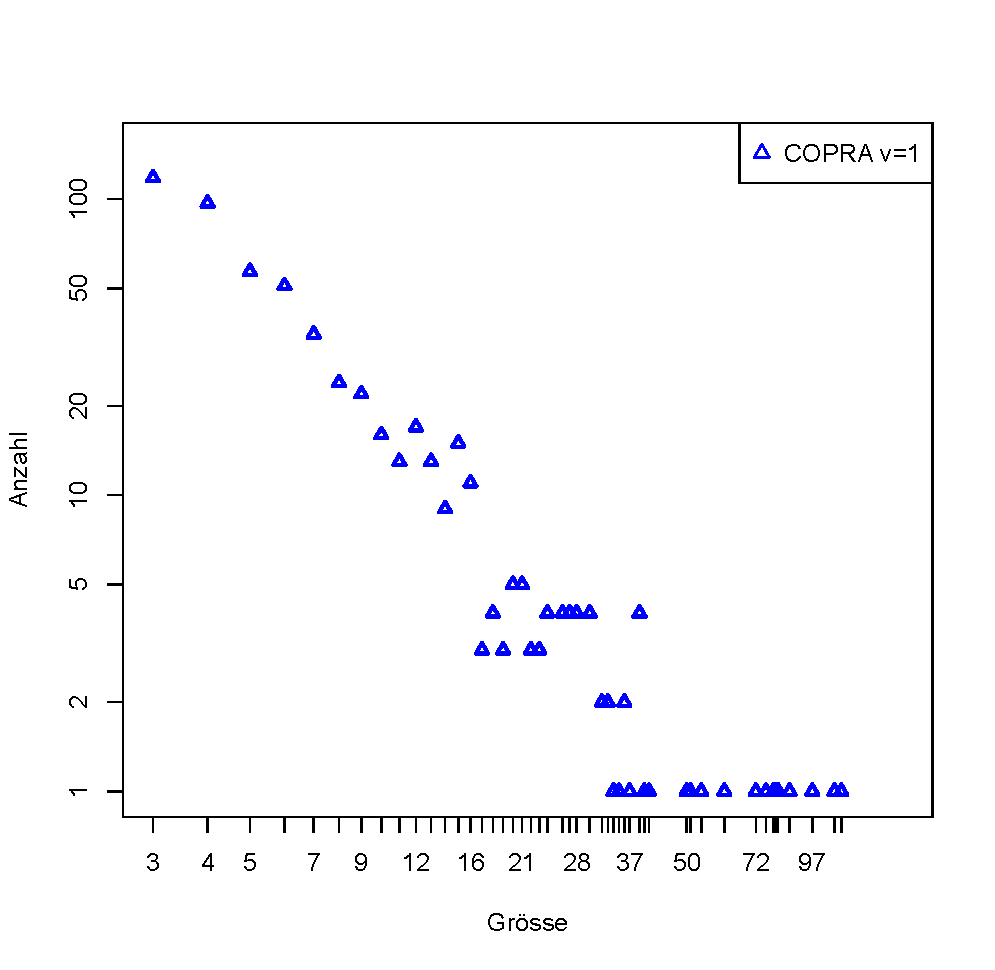
\includegraphics[scale=0.45]{images/time-corr_copra1.pdf}}
  \subfloat[]{\label{fig:time-corr-bl2} 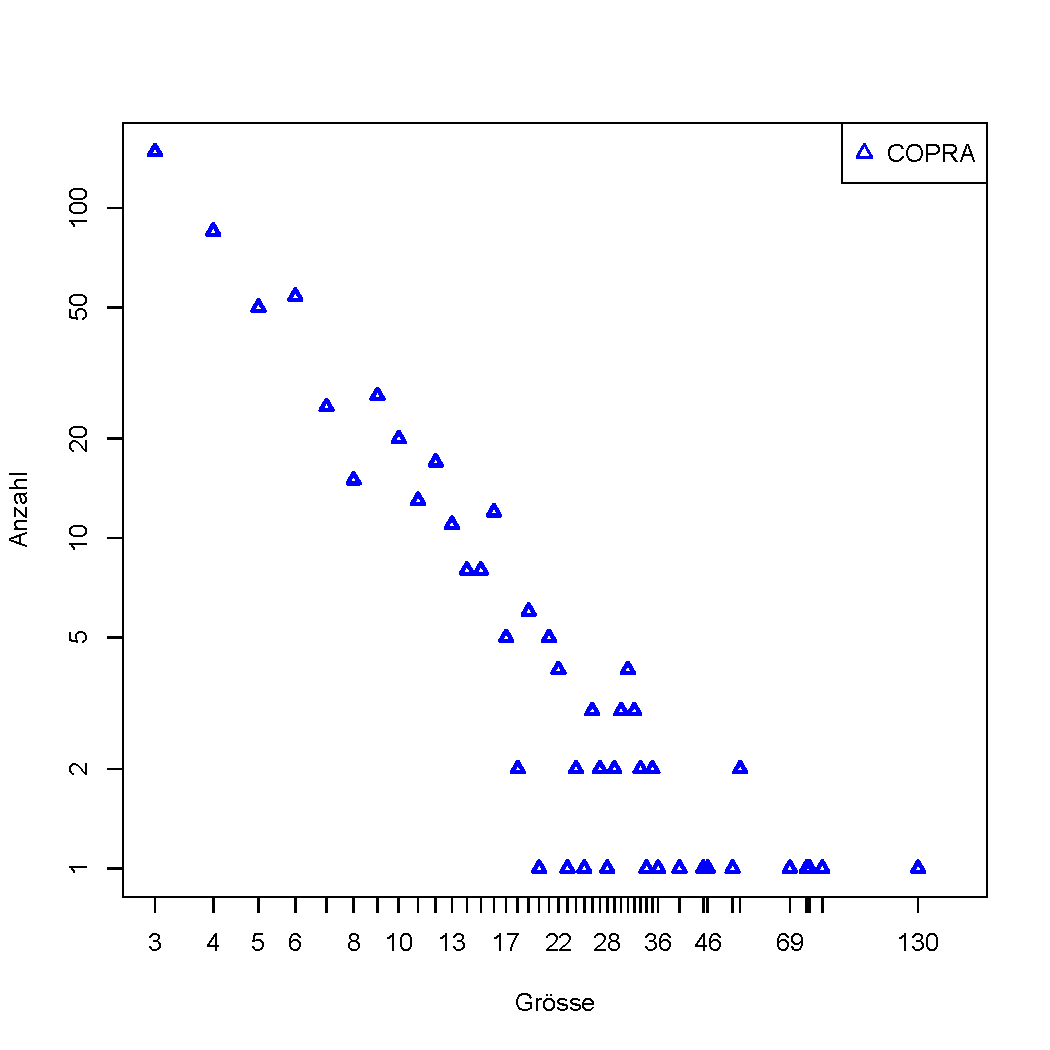
\includegraphics[scale=0.45]{images/time-corr_copra.pdf}}\\
  \subfloat[]{\label{fig:time-corr-bl5} 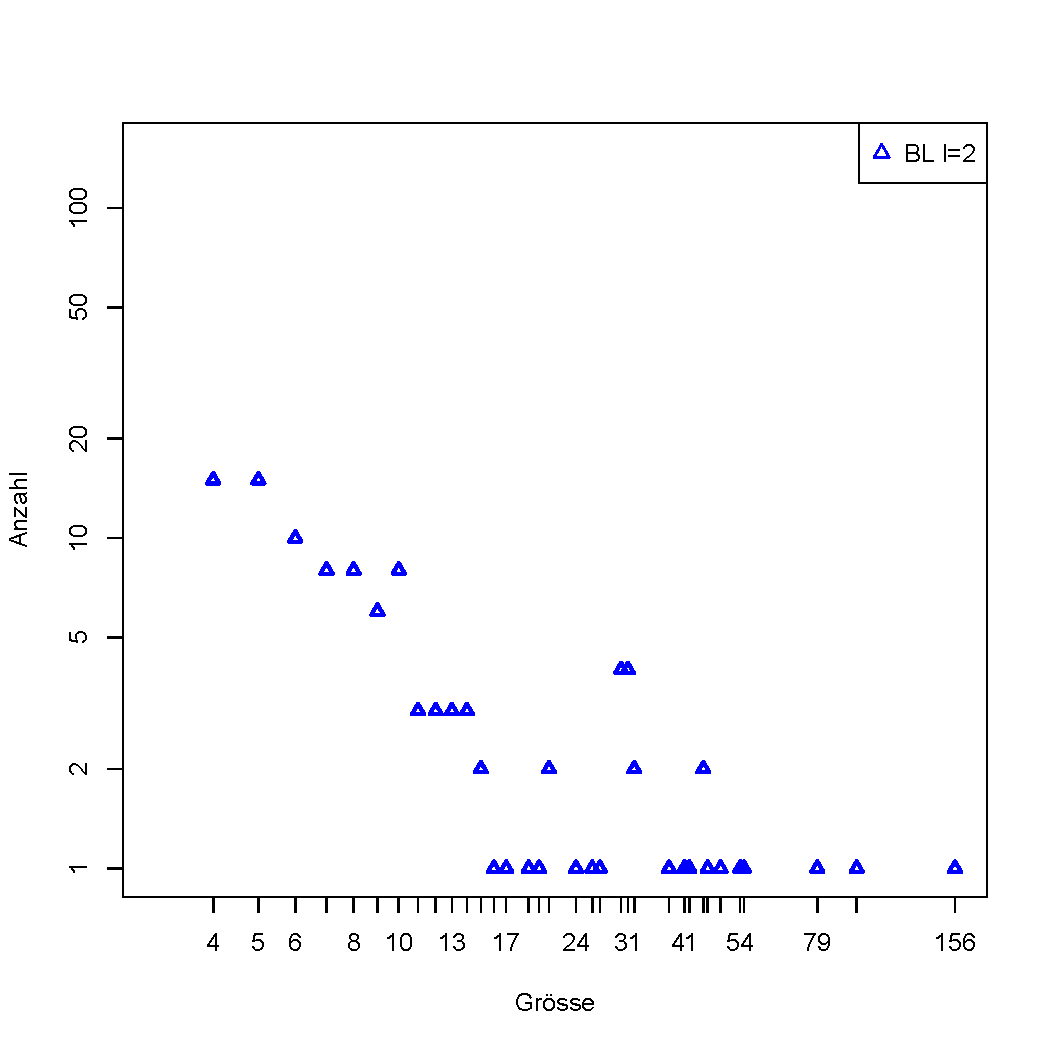
\includegraphics[scale=0.45]{images/time-corr_bl2.pdf}} 
  \subfloat[]{\label{fig:time-corr-copra} 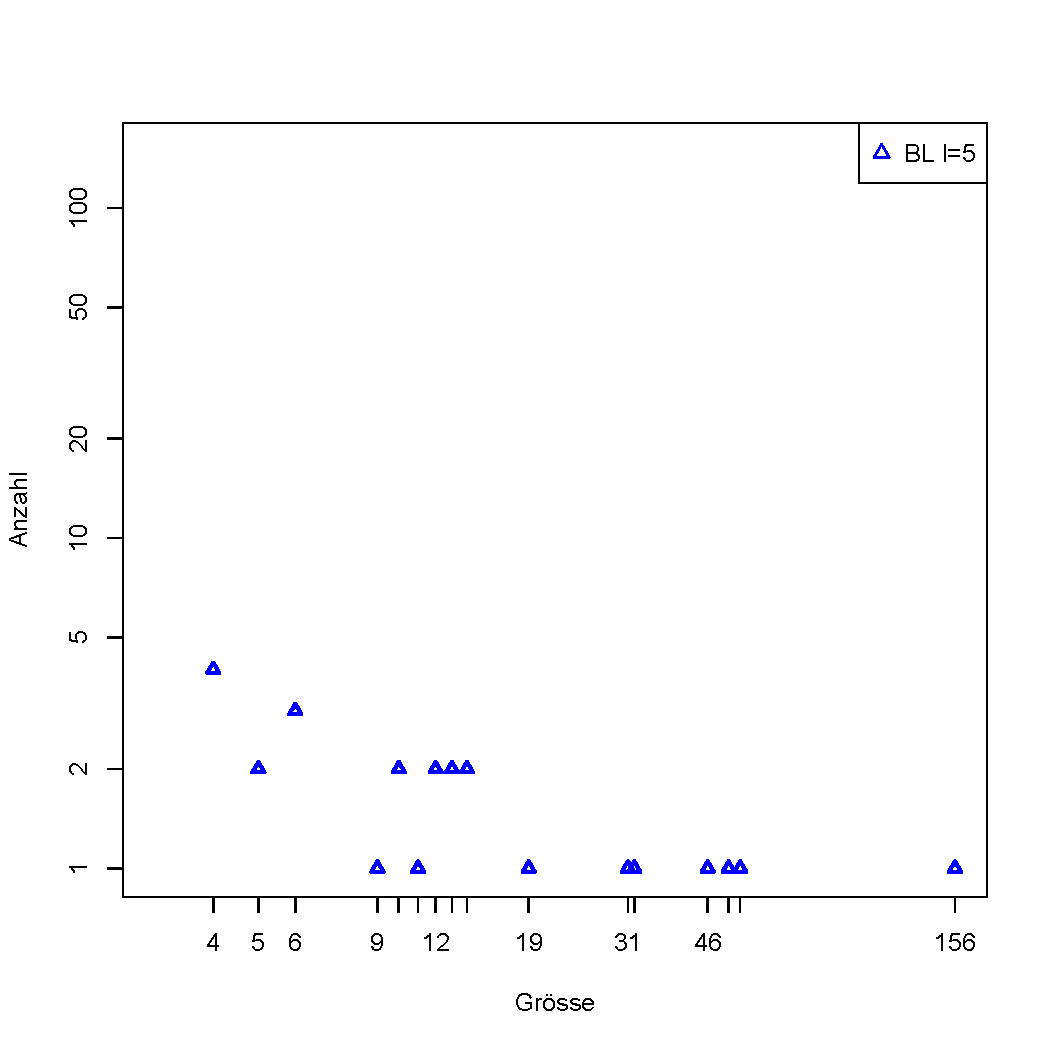
\includegraphics[scale=0.45]{images/time-corr_bl5.pdf}}
  \caption{Verteilung der Größe von Communities mit zeitlicher
    Korrelation der Signaturen.}
  \label{fig:time-corrdist}
\end{figure}

\subsection{Diskussion}
\label{sec:gesamtb-comm}

Diese Ergebnisse widerlegen nicht die Annahme, dass die Vernetzung im
Web of Trust im wesentlichen von Keysigning-Parties und den sozialen
Kontakten der Teilnehmer beeinflusst wird und damit unter anderem von
Gruppenzugehörigkeit bestimmt wird. Allerdings muss festgehalten
werden, dass die hier verwendeten Methoden nicht geeignet sind, um den
Entstehungsmechanismus entlang dieser Annahme befriedigend zu
erklären. 

Ein Grund dafür ist sicherlich, dass die Struktur des Web of Trust nur
zu einem bestimmten, festen Zeitpunkt betrachtet wurde. Um die
Entstehungsdynamik zu verstehen, könnte alternativ die Entwicklung des
Netzwerks tatsächlich über die Zeit nachvollzogen werden. Das
Keyserver-Netzwerk speichert nicht nur den momentanen Zustand des
Netzwerks, sondern implizit auch den Entstehungszeitpunkt jedes
Schlüssels und jeder Signatur. Die im Rahmen dieser Arbeit entwickelte
Software speichert diese Zeitstempel in einer Datenbank und macht so
die gesamte Entwicklungsgeschichte des Web of Trust verfügbar (siehe
Abschnitt \ref{sec:software}). Anhand dieser Daten könnte
nachvollzogen werden, wie und in welcher Form die Communities
tatsächlich entstehen und sich entwickeln.

Dass nur sehr wenige grö{\ss}ere Communities mit zeitlicher Korrelation
der Signaturen gefunden wurden, obwohl regelmäßig grö{\ss}ere
Keysigning-Parties stattfinden (siehe Abschnitt
\ref{sec:sozi-komp-des}) ist bei näherer Betrachtung durchaus
plausibel. Dass eine Keysigning-Party sich in der Struktur markant
abhebt, setzt voraus, dass ihre Teilnehmer außer der Teilnahme an
dieser Party keine wesentliche Signaturaktivität starten. Würden
sie weiterhin an Signaturaktitiväten teilnehmen, würde die
Struktur der Keysigning-Party mit der Zeit durch Signaturen von und zu
Nicht-Teilnehmern "`verwischt"' werden. Aufgefunden wurden also
vermutlich nur die Keysigning-Parties mit einer Mehrheit von insgesamt
eher inaktiven Teilnehmern. Gleiches kann für Teilnehmer angenommen
werden, die sich anhand von Gruppenzugehörigkeit vernetzen. Auch
hier würde die Struktur mit der Zeit "`unschärfer"' werden, wenn
ihre Mitglieder weiterhin Signierungen vornehmen würden. Es kann
also angenommen werden, dass die kleineren und insbesondere die klar
zuordnenbaren Communities tendenziell Teilnehmer enthalten, die in
Bezug auf die Teilnahme am Web of Trust eher inaktiv sind. Um diese
Vermutung zu bestätigen oder zu widerlegen, könnte das
Signaturverhalten der Teilnehmer über die Zeit mit ihrer
Community-Mitgliedschaft verglichen und korreliert werden.

Es scheint unrealistisch, dass die Mitgliedschaft in einer Gruppe --
etwa einer Firma, akademischen Einrichtung oder einem
Open-Source-Projekt -- die sozialen Kontakte einer Person
vollständig charakterisiert. Daneben kann eine Person noch ein
weites Netzwerk an Freunden oder Bekannten haben, die diese
Mitgliedschaft nicht teilen. Trotzdem können sich zu ihnen
Signaturen ergeben, die einen wesentlichen Teil der Signaturen dieser
Person ausmachen können. Außerdem ist anzunehmen, dass eine
Vielzahl solcher Gruppen nicht über eine gemeinsame Domain
verfügen, und damit mit den hier vorliegenden Daten schlicht nicht
sichtbar sind. Zwar wurde versucht, der anzunehmenden Komplexität
der Gruppenzugehörigkeiten durch überlappende Communities zu
begegnen. Allerdings konnte der verwendete Algorithmus keine
signifikanten Überlappungseigenschaften liefern. Die Frage,
inwiefern sich die einzelnen Communities sozialen Gruppen zuordnen
lassen, konnte also nur unvollständig beantwortet werden.

Es zeigt sich, dass dem Web of Trust kein einzelner, einfacher
Entstehungsmechanismus der hier angenommenen Form zugrunde liegt. Es
kann nur unzureichend beschrieben werden als eine Ansammlung von
einzelnen, einfach entstandenen Bausteinen, als die hier Communities
angenommen wurden. Implizit vorausgesetzt wird dabei auch, dass diese
zum Beispiel im Fall einer Keysigning-Party nach ihrer Entstehung
keine wesentliche weitere Vernetzungsaktitivät zeigen. Zwar trifft
dies für einen Teil der Communities -- gerade die, die eine
zeitliche Korrelation der Signaturen zeigen oder einer
Second-Level-Domain zugeordnet werden können -- durchaus zu. Für
einen erheblichen Anteil der Teilnehmer -- beispielsweise die
Mitglieder der sehr großen Community aus der COPRA-Berechnung --
scheint die Vernetzung jedoch so vielfältig zu sein, dass solche
einfachen Mechanismen nicht mehr sichtbar sind und "`in der Masse
verschwinden"'. Bei der COPRA-Zerlegung ist es etwa naheliegend, dass
die sehr große zentrale Community die Mehrzahl der aktiveren
Teilnehmer enthält. Hier ergibt sich eine Ähnlichkeit zur Struktur
der Zusammenhangskomponenten, bei denen die größte alle 
einigermaßen aktiven Teilnehmer zu enthalten scheint (siehe Abschnitt
\ref{sec:result-komponentenstruktur}).

Diese Punkte können anhand des Beispiels von Debian illustriert
werden: Das Debian-Projekt als tatsächliche Community, in der PGP
und das Web of Trust eine besonders wichtige Rolle spielen (siehe
Abschnitt \ref{sec:sozi-komp-des}) findet sich in den Zerlegungen
nicht als eigene abgegrenzte Einheit wieder. Statt dessen finden sich
sehr große Communities, in denen Debian-Entwickler einen signifikanten
Anteil der Schlüssel stellen. Im Fall der COPRA-Zerlegung ist dies
die bereits erwähnte Community mit ca. 21.000 Mitgliedern. Von
diesen verfügen 1.247 über eine E-Mail-Adresse in der Domain
debian.org und sind damit offensichtlich Mitglieder des
Debian-Projekts. Daneben finden sich Mitglieder des Debian-Projekts in
einer Vielzahl von kleineren Communities aller Größen. Die
Mitgliedschaft im Debian-Projekt scheint hier also für die
Vernetzung keine so wesentliche Rolle zu spielen, dass sie die
Struktur dieser real existierenden Community im Web of Trust
wieder spiegelt. Selbst wenn viele Debian-Entwickler mit vielen anderen
Projektmitgliedern vernetzt sind, so verfügen sie offensichtlich
über genügend andere Kontakte, so dass die sich aus den
projektinternen Kontakten ergebende Struktur nicht mehr
sichtbar ist.

\section{Zeitliche Entwicklung des Schlüsselbestandes}
\label{sec:result-key-properties}

\begin{figure}[th!]
  \centering
  \subfloat[]{\label{fig:size-dev-whole} \includegraphics[scale=0.3]{images/whole-size-time.pdf}}
  \subfloat[]{\label{fig:size-dev-mscc} \includegraphics[scale=0.3]{images/mscc-size-time.pdf}}
  \caption{Zeitliche Entwicklung der Größe des gesamten
    Schlüsselbestandes \subref{fig:size-dev-whole} und der
      grö{\ss}ten starken Zusammenhangskomponente \subref{fig:size-dev-mscc}}
  \label{fig:size-dev}
\end{figure}

Da die verwendete Datenbank alle jemals auf einen Keyserver geladenen
Schlüssel enthält, ist es möglich, den Zustand des Schlüsselbestandes
zu einem beliebigen Zeitpunkt zu berechnen. In Abbildung
\ref{fig:size-dev-whole} wird die Entwicklung der Größe des gesamten
Schlüsselbestandes und in \ref{fig:size-dev-mscc} die Entwicklung der
Größe der größten starken Zusammenhangskomponente dargestellt. Als
Beginn wurde das Jahr 1991 gewählt, da in diesem Jahr die erste
Version von PGP vorgestellt wurde (siehe Abschnitt
\ref{ch:Grundlagen:sec:PGP}). Sowohl der gesamte Schlüsselbestand als
auch die größte starke Zusammenhangskomponente zeigen nennenswertes
Wachstum erst etwa ab dem Jahr 1997. Dieser Zeitpunkt korreliert unter
anderem mit der Gründung des Unternehmens \emph{PGP Inc.}, der
Veröffentlichung einer neuen Version 5 der PGP-Software und in
Deutschland dem Start der bereits erwähnten
"`Krypto-Kampagne"'. Gründe für das deutlich langsamere Wachstum des
gesamten Schlüsselbestandes etwa ab dem Jahr 2001 und der größten
starken Zusammenhangskomponente mit einer Verzögerung etwa ab dem Jahr
2005 sind nicht bekannt. Es kann aber spekuliert werden, dass die
Zielgruppe, in der sich PGP/GnuPG prim\"ar verbreitet, begrenzt ist
(Anwender und Entwickler von freier Software, Sicherheitsexperten,
politische Aktivisten) und in dieser Zielgruppe eine gewisse
S\"attigung eingetreten ist. Ebenfalls m\"oglich ist eine zunehmende
Verbreitung von auf X.509 basierenden S/MIME-Zertifikaten.

\begin{figure}[th!]
  \centering
  \subfloat[]{\label{fig:pkalg-whole} 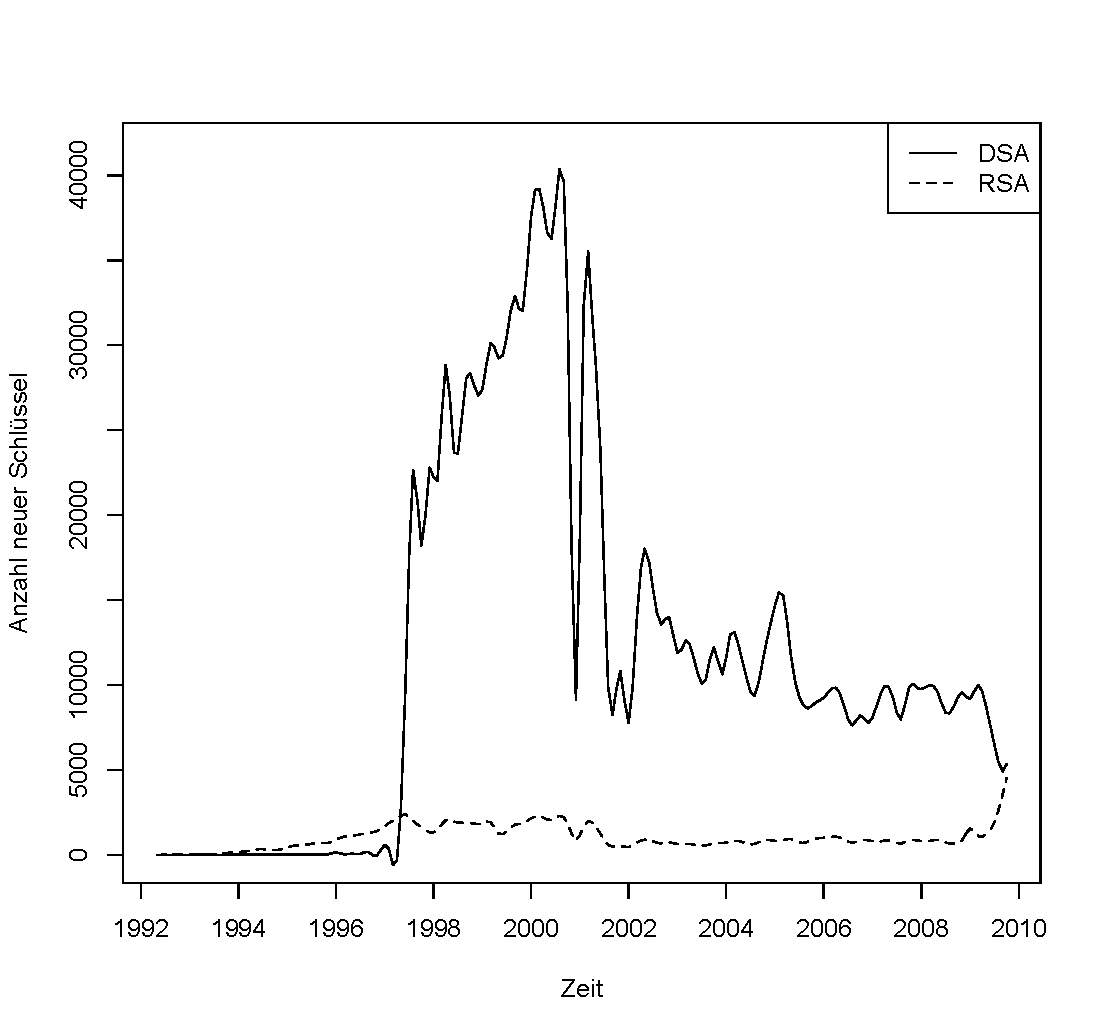
\includegraphics[scale=0.4]{images/whole-pkalg-use.pdf}}
  \subfloat[]{\label{fig:pkalg-mscc} 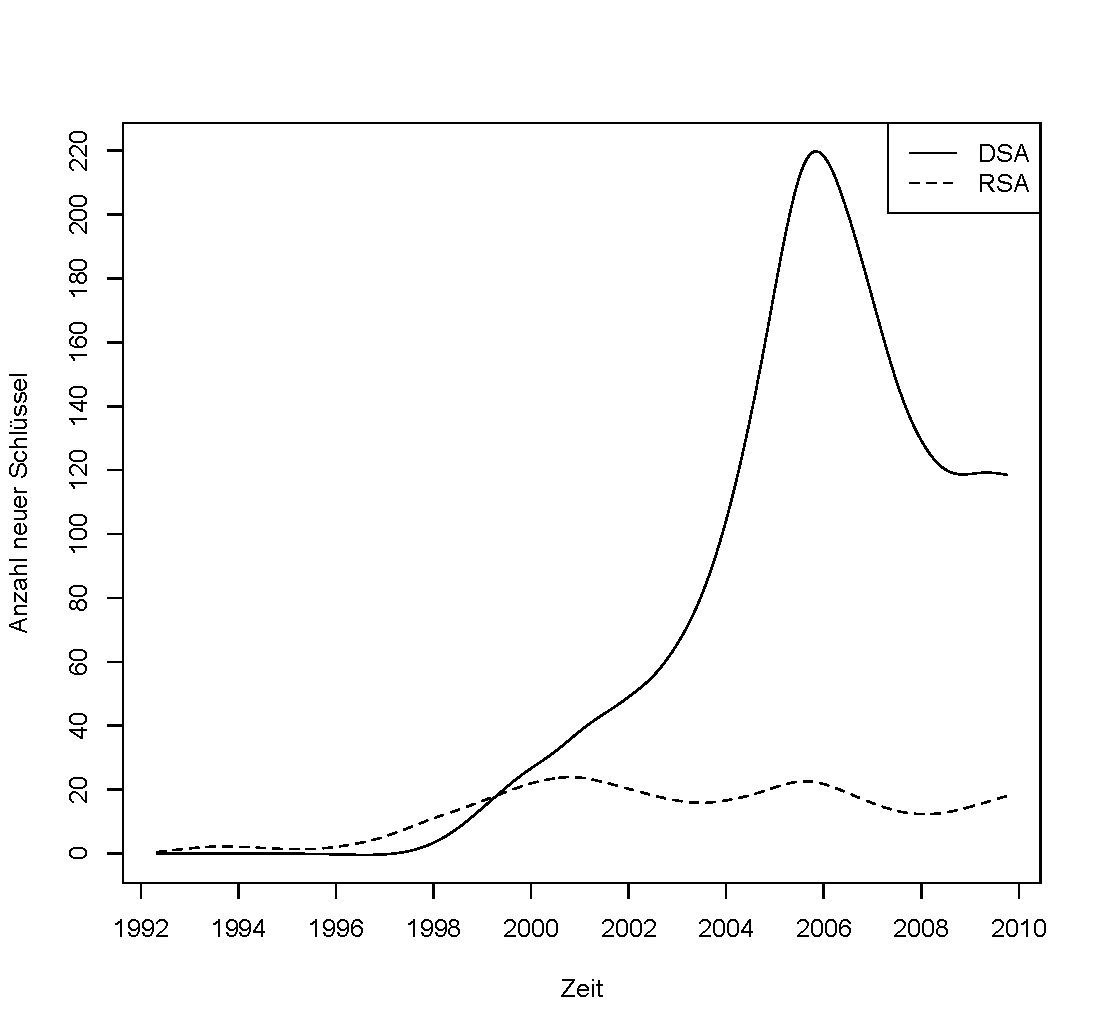
\includegraphics[scale=0.4]{images/mscc-pkalg-use.pdf}}
  \caption{Rate neuer PGP-Schlüssel, die RSA oder DSA benutzen,
    für den gesamten Schlüsselbestand \subref{fig:pkalg-whole} und
    die größte starke Zusammenhangskomponente
    \subref{fig:pkalg-mscc} in monatlichen Abständen}
  \label{fig:pkalg}
\end{figure}

Abbildung \ref{fig:size-dev} zeigt die Rate neuer Schlüssel,
abhängig von dem verwendeten Public-Key-Algorithmus. Die
DSA-Schlüssel\footnote{Mit DSA-Schlüssel sind hier öffentliche
  OpenPGP-Schlüssel gemeint, deren Public-Key-Paket
  DSA-Schlüsselmaterial enthält. Da DSA nicht zur
  Verschlüsselung benutzt werden kann, enthalten diese Schlüssel
  noch einen Unterschlüssel mit ElGamal-Schlüsselmaterial, der zum
  Verschlüsseln benutzt wird.} machen zu jedem Zeitpunkt den
größten Anteil aus. Ihre Entwicklung spiegelt im Wesentlichen die
Entwicklung der Größe insgesamt aus Abbildung \ref{fig:size-dev}
wieder. Demgegenüber ist die Zuwachsrate von RSA-Schlüsseln bis
zum Jahr 2008 konstant niedrig. Der Grund dafür ist vermutlich, dass
die PGP-Implementierungen in diesem Zeitraum in der
Standardeinstellung DSA-Schlüssel erzeugten, was wiederum unter
anderem in dem bis ins Jahr 2000 bestehenden Patentschutz des
RSA-Algorithmus begründet ist.  Die Rate neuer DSA-Schlüssel sinkt
ab dem Jahr 2009 deutlich ab, während die Rate neuer RSA-Schlüssel
gleichzeitig deutlich ansteigt. Vermutlich ist dies darauf
zurückzuführen, dass seit dem Jahr 2009 neue Schlüssel, die mit
GnuPG erzeugt werden, in der Standardeinstellung RSA statt DSA
verwenden. Diese Umstellung wurde in der Entwicklerversion von GnuPG
am
17.05.2009\footnote{http://lists.gnupg.org/pipermail/gnupg-devel/2009-May/025079.html}
aufgrund von Berichten über verbesserte Angriffe auf die
Hashfunktion SHA1 \cite{McDonald2009}, auf der DSA basiert,
vorgenommen. Warum diese Entwicklung nicht ebenfalls in der größten
starken Zusammenhangskomponente sichtbar ist, ist nicht
klar. Möglicherweise liegt dies daran, dass für die Aufnahme in
diese Teilmenge nicht nur das Erzeugen eines Schlüssels, sondern
auch zusätzliche Aktivität in Form der Vernetzung mit anderen
Schlüsseln notwendig ist. Neue Schlüssel werden also vermutlich im
Allgemeinen nicht sofort in die Zusammenhangskomponente aufgenommen,
sondern erst mit einiger Verzögerung. Die Zusammenhangskomponente
dürfte also etwas "`träger"' auf Veränderungen reagieren.

\section{Verwendung von Public-Key- und Hashalgorithmen}
\label{sec:public-key-und}

\begin{table}[ht!]
  \footnotesize
  \centering
  \subfloat[][]{
    \label{tab:hash}
    \begin{tabular}[ht!]{l|c}
      Algorithmus & Anzahl \\
      \hline
      Signaturen gesamt & 446.325 \\
      MD5 & 41.700 \\
      SHA1 & 398.849 \\
      RIPE-MD/160 & 122 \\
      SHA256 & 5.031 \\
      SHA512 & 2.472 \\
      SHA224 & 532
    \end{tabular}
  }\quad
  \subfloat[][]{
  \label{tab:algs}
    \begin{tabular}{l|c}
      Algorithmus & Anzahl \\
      \hline
      Schlüssel gesamt & 44.952 \\
      RSA-512 & 203 \\
      RSA-768 & 257 \\
      RSA-1024 & 3.903 \\
      RSA-2048 & 2.408 \\
      RSA-3072 & 96 \\
      RSA-4096 & 1.198 \\
      DSA & 36.555
    \end{tabular}
  }\quad
  \subfloat[][]{
    \label{tab:cert}
    \begin{tabular}{l|c}
      Cert Level & Anzahl \\
      \hline
      Signaturen gesamt & 446.325 \\
      Generic & 299.518 \\
      Persona & 904 \\
      Casual & 28.718 \\
      Positive & 119.575 
    \end{tabular}
  }
  \caption{Verwendung von Hashalgorithmen 
    \subref{tab:hash}, Public-Key-Algorithmen \subref{tab:algs} und
    certification levels \subref{tab:cert} in der grössten starken
    Zusammenhangskomponente}
\end{table}

In Tabelle \ref{tab:algs} sind schlussendlich noch einige Statistiken
über Eigenschaften einzelner Schlüssel aufgeführt. 

Die einzelnen "`certification level"' (siehe Abschnitt
\ref{sec:das-gnupg-vertrauensmodell}) werden durchaus verwendet
(Tabelle \ref{tab:cert}). Zwar ist die Mehrheit der Signaturen mit
dem Standardwert "`Generic"' versehen, der keine weitere Aussage
macht. Allerdings verfügen über 25\% der Signaturen über den
höchsten Wert "`Positive"'. Da die Level keine im Standard
festgelegte klare Semantik haben, ist die Aussagekraft dieser Werte
natürlich begrenzt. Sie können aber zumindest dahingehend
interpretiert werden, dass \emph{mindestens} die Personen, die von
"`Generic"' abweichende Werte vergeben, den Signaturprozess durchaus
ernst nehmen.

Wie zu erwarten basiert die große Mehrheit der Signaturen in der
größten starken Zusammenhangskomponente auf SHA1. Neben einzelnen
Signaturen mit Vertretern der SHA2-Familie findet sich aber auch noch
eine überraschend hohe Anzahl von MD5-Signaturen: 41.700 Signaturen,
d.h. 10\% basieren auf MD5. Die Sicherheit von MD5 muss inzwischen als
ernsthaft kompromittiert eingestuft werden. 2008 gelang es einer
Gruppe, durch eine Chosen-Prefix-Kollision ein von einer kommerziellen
CA signiertes "`bösartiges"' Certification-Authority-Zertifikat
für SSL zu erhalten \cite{Stevens2009}. GnuPG warnt zwar vor der
Verwendung von MD5-Signaturen, erlaubt ihre Verwendung aber noch. Die
Bedeutung der MD5-Signaturen für den Zusammenhalt der größten
Komponente ist nicht unwesentlich: Werden diese Signaturen entfernt,
reduziert sich die Größe der Komponente auf 37.599 Schlüssel,
d.h. es werden ca. 8.000 Schlüssel abgetrennt. 

RSA-Schlüssel mit einer Länge von höchstens 768 Bit und weniger
müssen ebenfalls als praktikabel brechbar betrachtet werden. Dies
wurde durch die Faktorisierung der Zahl RSA-768 demonstriert
\cite{Kleinjung2010}. Kleinjung et al. schätzen den Zeitrahmen bis
zur Faktorisierung einer 1024-Bit-Zahl innerhalb eines
\emph{akademischen Rahmens} auf 5 bis 10 Jahre. Die Menge der in der
größten Komponente vorhandenen RSA-Schlüssel mit 512 bzw. 768 Bit
ist mit insgesamt 450 Schlüsseln gering. Ihre Entfernung trennt nur
etwa weitere 300 Knoten von der Komponente ab. Die Anzahl von
RSA-Schlüsseln mit 1024 Bit ist aber deutlich größer. Die
Entfernung aller ca. 4.500 RSA-Schlüssel, deren Länge höchstens
1024 Bit beträgt, reduziert die Größe der Komponente um insgesamt
ca. 8.500 Knoten, trennt also weitere 4.000 Knoten vom Netz ab. Es ist
anzunehmen, dass sich die durchschnittlichen Distanzen ebenfalls
erhöhen. Da die Standardisierungsorganisation \emph{National Institute
 of Standards and Technology} 
  eine Abkehr von RSA-1024
ab dem Jahr 2010 empfiehlt \cite{NIST2007} und praktikable Angriffe
wohl nur eine Frage weniger Jahre sind, ist damit wie durch die
MD5-Signaturen eine erhebliche Beeinträchtigung der größten
Komponente absehbar.

Es ist zu erwarten, dass sich durch die Umstellung der
Standardeinstellung in GnuPG der Anteil von RSA-Schlüsseln mit
einer Länge von mindestens 2048 bit in nächster Zeit deutlich
erhöht.

%% ==============================
\section{Verwandte Arbeiten}
%% ==============================
\label{ch:Grundlagen:sec:RelatedWork}

An dieser Stelle wird nur auf Arbeiten eingegangen, die sich mit der
Netzwerkstruktur des Web of Trust bei PGP beschäftigen. Für einen
Überblick über Arbeiten zur Struktur von anderen Netzwerken sei auf
\cite{newman:167} und für Arbeiten zur Community-Struktur von anderen
Netzwerken auf \cite{Fortunato2010} verwiesen.

Capkun et al. \cite{Capkun2002} untersuchten strukturelle Aspekte der
größten starken Zusammenhangskomponente eines PGP-Netzwerkes aus dem
Jahr 2001. Dieses Netzwerk zeigte eine geringe charakteristische
Distanz und einen hohen Clustering-Koeffizienten. Außerdem stimmte die
Verteilung der aus- und eingehenden Grade mit einem Power-Law
überein. Die Autoren argumentieren, dass Netzwerke, die aus
Zertifikatsbeziehungen entstehen, naturgemäß den Small-World-Effekt
zeigen, da sich die Zertifikate anhand schon bestehender
Vertrauensbeziehungen ergeben. Die Autoren geben außerdem noch ein
Netzwerkmodell an, das Graphen erzeugen soll, die in den
beschriebenen Charakteristiken dem PGP-Netzwerk ähneln.

Arenas et al. \cite{Boguna2004} analysierten ein PGP-Netzwerk aus dem
gleichen Jahr. Das Netzwerk wurde von vornherein in ein ungerichtetes
Netzwerk umgewandelt, indem nicht gegenseitige Kanten entfernt
wurden. Sie betrachteten die Gradverteilung, den
Clustering-Koeffizienten und die Korrelation von Graden benachbarter
Knoten. Dabei folgt die Verteilung der Knotengrade einem
Power-Law. Der Clustering-Koeffizient des Netzwerkes beträgt $C=0.4$,
ist also recht hoch. Die Grade benachbarter Knoten sind positiv
korreliert. Außerdem benutzten die Autoren den Algorithmus von Girvan
und Newman \cite{Newman2004}, um eine Community-Zerlegung des Netzwerks
zu berechnen. Die Verteilung der Größe dieser Communities folgt wieder
einem Power-Law.

Warren et al. betrachteten das Netzwerk nicht zu einem festen
Zeitpunkt sondern untersuchten die \emph{Dynamik} des
Netzwerks \cite{Warren2007}. Sie berechneten verschiedene grundlegende
Netzwerkeigenschaften (Größe des Netzwerkes, Distanzen,
Gradverteilung etc.) und verfolgten deren Entwicklung \emph{über die
  Zeit}. Ihre Ergebnisse können allerdings mit den in dieser Arbeit
präsentierten nicht sinnvoll verglichen werden, da der Graph von Schlüsseln
auf Individuen reduziert wurde (siehe auch Abschnitt
\ref{sec:schl-und-invid}).

Gemein ist diesen akademischen Arbeiten, dass sie auf deutlich
\"alteren Datens\"atzen beruhen. Insbesondere bei \cite{Capkun2002}
und \cite{Boguna2004} kamen Daten aus dem Jahr 2001 zum
Einsatz. Seither hat sich die MSCC von ca. 12.000 auf ca. 45.000 Knoten
vergr\"ossert. Bei einer Ver\"anderung diesen Ausma{\ss}es kann nicht
von vornherein ausgeschlossen werden, dass sich grundlegende Merkmale
des Netzwerks ver\"andert haben. Schon aus diesem Grund scheint es
berechtigt, dass in dieser Arbeit Merkmale untersucht wurden, die auch
schon in fr\"uhren Arbeiten betrachtet wurden. Au{\ss}erdem
wurde diese Arbeit in Bezug auf die untersuchten Merkmale deutlich
breiter angelegt.

Neben diesen akademischen Arbeiten gibt es mehrere Ansätze aus der
PGP-Community, die Netzwerkstruktur zu untersuchen. Das
wotsap-Projekt \cite{Cederlof} stellt einen täglich aktualisierten
Datensatz bereit, der die Vernetzungsstruktur der größten starken
Zusammenhangskomponente des Web of Trust darstellt. Diese Daten werden
für eine Webapplikation benutzt, die kürzeste Pfade
zwischen Schlüsseln berechnet und visualisiert und so bei der
Nutzung von Zertifikatspfaden behilflich sein soll. In Abschnitt
\ref{ch:Grundlagen:sec:WarumEigene} wird der Wotsap-Datensatz näher
betrachtet und begründet, warum er in dieser Arbeit nicht verwendet
wurde. 

Henk P. Penning berechnet anhand der Wotsap-Daten regelmäßig
strukturelle Eigenschaften des Web of Trust bzw. von dessen größter
starker Zusammenhangskomponente \cite{Penning}. Dies beinhaltet die
Entwicklung der Größe dieser Komponente und der durchschnittlichen
Distanzen über die Zeit, die Verteilung der Knotengrade und die
Verteilung durchschnittlicher Distanzen pro Knoten. Außerdem wird die
Robustheit des Netzwerkes bei der Entfernung von zufällig
ausgewählten bzw. besonders gut vernetzten Knoten simuliert.

In allen Arbeiten zeigen die betrachteten Netzwerke konsistente
Eigenschaften, die auch mit den Ergebnissen dieser Arbeit
\"ubereinstimmen. Dies sind im wesentlichen die charakteristischen
Merkmale eines sozialen Netzwerks: Eine niedrige charakteristische
Distanz, ein hohes Ausma{\ss} an Clustering und eine pr\"agnante
Zusammenballung von Knoten in Communities. Ausserdem \"ahneln sich die
Verteilungen der Knoten insofern, als sie einer Power-Law-Verteilung
zumindest \emph{\"ahneln}. Diese grundlegenden Merkmale haben sich
also trotz des deutlichen Wachstums der Knotenanzahl qualitativ nicht
ver\"andert. 

%%% Local Variables: 
%%% mode: latex
%%% TeX-master: "diplarb"
%%% End: 

